% Options for packages loaded elsewhere
% Options for packages loaded elsewhere
\PassOptionsToPackage{unicode}{hyperref}
\PassOptionsToPackage{hyphens}{url}
\PassOptionsToPackage{dvipsnames,svgnames,x11names}{xcolor}
%
\documentclass[
  letterpaper,
  DIV=11,
  numbers=noendperiod]{scrartcl}
\usepackage{xcolor}
\usepackage[top=30mm,left=30mm]{geometry}
\usepackage{amsmath,amssymb}
\setcounter{secnumdepth}{-\maxdimen} % remove section numbering
\usepackage{iftex}
\ifPDFTeX
  \usepackage[T1]{fontenc}
  \usepackage[utf8]{inputenc}
  \usepackage{textcomp} % provide euro and other symbols
\else % if luatex or xetex
  \usepackage{unicode-math} % this also loads fontspec
  \defaultfontfeatures{Scale=MatchLowercase}
  \defaultfontfeatures[\rmfamily]{Ligatures=TeX,Scale=1}
\fi
\usepackage{lmodern}
\ifPDFTeX\else
  % xetex/luatex font selection
\fi
% Use upquote if available, for straight quotes in verbatim environments
\IfFileExists{upquote.sty}{\usepackage{upquote}}{}
\IfFileExists{microtype.sty}{% use microtype if available
  \usepackage[]{microtype}
  \UseMicrotypeSet[protrusion]{basicmath} % disable protrusion for tt fonts
}{}
\makeatletter
\@ifundefined{KOMAClassName}{% if non-KOMA class
  \IfFileExists{parskip.sty}{%
    \usepackage{parskip}
  }{% else
    \setlength{\parindent}{0pt}
    \setlength{\parskip}{6pt plus 2pt minus 1pt}}
}{% if KOMA class
  \KOMAoptions{parskip=half}}
\makeatother
% Make \paragraph and \subparagraph free-standing
\makeatletter
\ifx\paragraph\undefined\else
  \let\oldparagraph\paragraph
  \renewcommand{\paragraph}{
    \@ifstar
      \xxxParagraphStar
      \xxxParagraphNoStar
  }
  \newcommand{\xxxParagraphStar}[1]{\oldparagraph*{#1}\mbox{}}
  \newcommand{\xxxParagraphNoStar}[1]{\oldparagraph{#1}\mbox{}}
\fi
\ifx\subparagraph\undefined\else
  \let\oldsubparagraph\subparagraph
  \renewcommand{\subparagraph}{
    \@ifstar
      \xxxSubParagraphStar
      \xxxSubParagraphNoStar
  }
  \newcommand{\xxxSubParagraphStar}[1]{\oldsubparagraph*{#1}\mbox{}}
  \newcommand{\xxxSubParagraphNoStar}[1]{\oldsubparagraph{#1}\mbox{}}
\fi
\makeatother

\usepackage{color}
\usepackage{fancyvrb}
\newcommand{\VerbBar}{|}
\newcommand{\VERB}{\Verb[commandchars=\\\{\}]}
\DefineVerbatimEnvironment{Highlighting}{Verbatim}{commandchars=\\\{\}}
% Add ',fontsize=\small' for more characters per line
\usepackage{framed}
\definecolor{shadecolor}{RGB}{241,243,245}
\newenvironment{Shaded}{\begin{snugshade}}{\end{snugshade}}
\newcommand{\AlertTok}[1]{\textcolor[rgb]{0.68,0.00,0.00}{#1}}
\newcommand{\AnnotationTok}[1]{\textcolor[rgb]{0.37,0.37,0.37}{#1}}
\newcommand{\AttributeTok}[1]{\textcolor[rgb]{0.40,0.45,0.13}{#1}}
\newcommand{\BaseNTok}[1]{\textcolor[rgb]{0.68,0.00,0.00}{#1}}
\newcommand{\BuiltInTok}[1]{\textcolor[rgb]{0.00,0.23,0.31}{#1}}
\newcommand{\CharTok}[1]{\textcolor[rgb]{0.13,0.47,0.30}{#1}}
\newcommand{\CommentTok}[1]{\textcolor[rgb]{0.37,0.37,0.37}{#1}}
\newcommand{\CommentVarTok}[1]{\textcolor[rgb]{0.37,0.37,0.37}{\textit{#1}}}
\newcommand{\ConstantTok}[1]{\textcolor[rgb]{0.56,0.35,0.01}{#1}}
\newcommand{\ControlFlowTok}[1]{\textcolor[rgb]{0.00,0.23,0.31}{\textbf{#1}}}
\newcommand{\DataTypeTok}[1]{\textcolor[rgb]{0.68,0.00,0.00}{#1}}
\newcommand{\DecValTok}[1]{\textcolor[rgb]{0.68,0.00,0.00}{#1}}
\newcommand{\DocumentationTok}[1]{\textcolor[rgb]{0.37,0.37,0.37}{\textit{#1}}}
\newcommand{\ErrorTok}[1]{\textcolor[rgb]{0.68,0.00,0.00}{#1}}
\newcommand{\ExtensionTok}[1]{\textcolor[rgb]{0.00,0.23,0.31}{#1}}
\newcommand{\FloatTok}[1]{\textcolor[rgb]{0.68,0.00,0.00}{#1}}
\newcommand{\FunctionTok}[1]{\textcolor[rgb]{0.28,0.35,0.67}{#1}}
\newcommand{\ImportTok}[1]{\textcolor[rgb]{0.00,0.46,0.62}{#1}}
\newcommand{\InformationTok}[1]{\textcolor[rgb]{0.37,0.37,0.37}{#1}}
\newcommand{\KeywordTok}[1]{\textcolor[rgb]{0.00,0.23,0.31}{\textbf{#1}}}
\newcommand{\NormalTok}[1]{\textcolor[rgb]{0.00,0.23,0.31}{#1}}
\newcommand{\OperatorTok}[1]{\textcolor[rgb]{0.37,0.37,0.37}{#1}}
\newcommand{\OtherTok}[1]{\textcolor[rgb]{0.00,0.23,0.31}{#1}}
\newcommand{\PreprocessorTok}[1]{\textcolor[rgb]{0.68,0.00,0.00}{#1}}
\newcommand{\RegionMarkerTok}[1]{\textcolor[rgb]{0.00,0.23,0.31}{#1}}
\newcommand{\SpecialCharTok}[1]{\textcolor[rgb]{0.37,0.37,0.37}{#1}}
\newcommand{\SpecialStringTok}[1]{\textcolor[rgb]{0.13,0.47,0.30}{#1}}
\newcommand{\StringTok}[1]{\textcolor[rgb]{0.13,0.47,0.30}{#1}}
\newcommand{\VariableTok}[1]{\textcolor[rgb]{0.07,0.07,0.07}{#1}}
\newcommand{\VerbatimStringTok}[1]{\textcolor[rgb]{0.13,0.47,0.30}{#1}}
\newcommand{\WarningTok}[1]{\textcolor[rgb]{0.37,0.37,0.37}{\textit{#1}}}

\usepackage{longtable,booktabs,array}
\usepackage{calc} % for calculating minipage widths
% Correct order of tables after \paragraph or \subparagraph
\usepackage{etoolbox}
\makeatletter
\patchcmd\longtable{\par}{\if@noskipsec\mbox{}\fi\par}{}{}
\makeatother
% Allow footnotes in longtable head/foot
\IfFileExists{footnotehyper.sty}{\usepackage{footnotehyper}}{\usepackage{footnote}}
\makesavenoteenv{longtable}
\usepackage{graphicx}
\makeatletter
\newsavebox\pandoc@box
\newcommand*\pandocbounded[1]{% scales image to fit in text height/width
  \sbox\pandoc@box{#1}%
  \Gscale@div\@tempa{\textheight}{\dimexpr\ht\pandoc@box+\dp\pandoc@box\relax}%
  \Gscale@div\@tempb{\linewidth}{\wd\pandoc@box}%
  \ifdim\@tempb\p@<\@tempa\p@\let\@tempa\@tempb\fi% select the smaller of both
  \ifdim\@tempa\p@<\p@\scalebox{\@tempa}{\usebox\pandoc@box}%
  \else\usebox{\pandoc@box}%
  \fi%
}
% Set default figure placement to htbp
\def\fps@figure{htbp}
\makeatother





\setlength{\emergencystretch}{3em} % prevent overfull lines

\providecommand{\tightlist}{%
  \setlength{\itemsep}{0pt}\setlength{\parskip}{0pt}}



 


\KOMAoption{captions}{tableheading}
\makeatletter
\@ifpackageloaded{tcolorbox}{}{\usepackage[skins,breakable]{tcolorbox}}
\@ifpackageloaded{fontawesome5}{}{\usepackage{fontawesome5}}
\definecolor{quarto-callout-color}{HTML}{909090}
\definecolor{quarto-callout-note-color}{HTML}{0758E5}
\definecolor{quarto-callout-important-color}{HTML}{CC1914}
\definecolor{quarto-callout-warning-color}{HTML}{EB9113}
\definecolor{quarto-callout-tip-color}{HTML}{00A047}
\definecolor{quarto-callout-caution-color}{HTML}{FC5300}
\definecolor{quarto-callout-color-frame}{HTML}{acacac}
\definecolor{quarto-callout-note-color-frame}{HTML}{4582ec}
\definecolor{quarto-callout-important-color-frame}{HTML}{d9534f}
\definecolor{quarto-callout-warning-color-frame}{HTML}{f0ad4e}
\definecolor{quarto-callout-tip-color-frame}{HTML}{02b875}
\definecolor{quarto-callout-caution-color-frame}{HTML}{fd7e14}
\makeatother
\makeatletter
\@ifpackageloaded{caption}{}{\usepackage{caption}}
\AtBeginDocument{%
\ifdefined\contentsname
  \renewcommand*\contentsname{Table of contents}
\else
  \newcommand\contentsname{Table of contents}
\fi
\ifdefined\listfigurename
  \renewcommand*\listfigurename{List of Figures}
\else
  \newcommand\listfigurename{List of Figures}
\fi
\ifdefined\listtablename
  \renewcommand*\listtablename{List of Tables}
\else
  \newcommand\listtablename{List of Tables}
\fi
\ifdefined\figurename
  \renewcommand*\figurename{Figure}
\else
  \newcommand\figurename{Figure}
\fi
\ifdefined\tablename
  \renewcommand*\tablename{Table}
\else
  \newcommand\tablename{Table}
\fi
}
\@ifpackageloaded{float}{}{\usepackage{float}}
\floatstyle{ruled}
\@ifundefined{c@chapter}{\newfloat{codelisting}{h}{lop}}{\newfloat{codelisting}{h}{lop}[chapter]}
\floatname{codelisting}{Listing}
\newcommand*\listoflistings{\listof{codelisting}{List of Listings}}
\makeatother
\makeatletter
\makeatother
\makeatletter
\@ifpackageloaded{caption}{}{\usepackage{caption}}
\@ifpackageloaded{subcaption}{}{\usepackage{subcaption}}
\makeatother
\usepackage{bookmark}
\IfFileExists{xurl.sty}{\usepackage{xurl}}{} % add URL line breaks if available
\urlstyle{same}
\hypersetup{
  pdftitle={Introduction to Collaborative Coding with GitHub},
  pdfauthor={Elizabeth Waterfield},
  colorlinks=true,
  linkcolor={blue},
  filecolor={Maroon},
  citecolor={Blue},
  urlcolor={Blue},
  pdfcreator={LaTeX via pandoc}}


\title{Introduction to Collaborative Coding with GitHub}
\author{Elizabeth Waterfield}
\date{04/03/2026}
\begin{document}
\maketitle


\subsection{Licence}\label{licence}

This work was originally created by
\href{https://github.com/annakrystalli}{Anna Krystalli} from
\href{https://github.com/RSE-Sheffield}{RSE-Sheffield} under a
\href{https://github.com/RSE-Sheffield/collaborative_github_exercise}{MIT
licence (original repository)}. It was subsequently adapted by
\href{https://ox.ukrn.org/people/\#MalikaIhle}{Malika Ihle} during her
time at \href{https://ox.ukrn.org/}{Reproducible Research Oxford}, with
the contributions of Adam Kenny. This work by Elizabeth Waterfield,
Sarah von Grebmer zu Wolfsthurn, and Malika Ihle is licensed under a
CC-BY-SA 4.0
\href{https://creativecommons.org/licenses/by-sa/4.0/deed.en}{Creative
Commons Attribution 4.0 International SA License}. It permits
unrestricted re-use, distribution, and reproduction in any medium,
provided the original work is properly cited. If you remix, transform,
or build upon the material, you must distribute your contributions under
the same license as the original.

\textbf{Presenter Notes}: The Creative Commons Attribution--ShareAlike
4.0 license, or CC BY-SA 4.0, allows others to copy, share, and adapt a
work in any medium, including for commercial purposes. These permissions
are broad and cannot be withdrawn as long as the license terms are
followed. The main requirement is attribution: users must give
appropriate credit to the original creator, provide a link to the
license, and clearly indicate whether any changes were made, without
implying endorsement by the original author. In addition, the ShareAlike
condition means that if someone modifies or builds upon the work, the
resulting material must be distributed under the same CC BY-SA 4.0
license, or a compatible one. Finally, users are not allowed to apply
legal or technical restrictions, such as DRM, that would prevent others
from exercising these same rights.

\begin{center}\rule{0.5\linewidth}{0.5pt}\end{center}

\subsection{Contribution statement}\label{contribution-statement}

\textbf{Creator}: Waterfield, Elizabeth
(\pandocbounded{
\includegraphics[keepaspectratio]{images/ORCID-iD_icon_16x16.png}}\href{https://orcid.org/0009-0006-3725-6730}{0009-0006-3725-6730})

\textbf{Reviewer}: von Grebmer zu Wolfsthurn, Sarah
(\pandocbounded{
\includegraphics[keepaspectratio]{images/ORCID-iD_icon_16x16.png}}\href{https://orcid.org/0000-0002-6413-3895}{0000-0002-6413-3895})

\textbf{Consultant}: Ihle, Malika
(\pandocbounded{
\includegraphics[keepaspectratio]{images/ORCID-iD_icon_16x16.png}}\href{https://orcid.org/0000-0002-3242-5981}{0000-0002-3242-5981})

\textbf{Presenter Notes}: Speaker notes may act as a guiding script for
delivering the presentation. These notes contain key information, such
as phrases, explanations, or transitions, that can be said aloud to
clarify concepts, emphasize important points, or maintain the flow of
information.

\textbf{Instructor Notes}: Instructor notes provide teaching support but
are not intended to be communicated to the learners directly. These
notes contain additional context, such as learning objectives, common
issues, and pedagogical tips, to help the instructor adapt their
teaching to the learner's needs as well as anticipate challenges.

\textbf{Acessibility Tips}: Where applicable, this is a space to add any
tips you may have to facilitate the accessibility of your slides and
activities.

\begin{center}\rule{0.5\linewidth}{0.5pt}\end{center}

\subsubsection{Prerequisites}\label{prerequisites}

\begin{tcolorbox}[enhanced jigsaw, colbacktitle=quarto-callout-important-color!10!white, opacityback=0, leftrule=.75mm, colback=white, opacitybacktitle=0.6, colframe=quarto-callout-important-color-frame, title=\textcolor{quarto-callout-important-color}{\faExclamation}\hspace{0.5em}{Prerequisites}, left=2mm, titlerule=0mm, toptitle=1mm, breakable, bottomtitle=1mm, arc=.35mm, rightrule=.15mm, bottomrule=.15mm, toprule=.15mm, coltitle=black]

Before completing this submodule, please carefully read about the
necessary prerequisites.

\end{tcolorbox}

\begin{longtable}[]{@{}
  >{\raggedright\arraybackslash}p{(\linewidth - 4\tabcolsep) * \real{0.3333}}
  >{\raggedright\arraybackslash}p{(\linewidth - 4\tabcolsep) * \real{0.3333}}
  >{\raggedright\arraybackslash}p{(\linewidth - 4\tabcolsep) * \real{0.3333}}@{}}
\toprule\noalign{}
\begin{minipage}[b]{\linewidth}\raggedright
Prerequisite
\end{minipage} & \begin{minipage}[b]{\linewidth}\raggedright
Description
\end{minipage} & \begin{minipage}[b]{\linewidth}\raggedright
Where to find it
\end{minipage} \\
\midrule\noalign{}
\endhead
\bottomrule\noalign{}
\endlastfoot
R and RStudio installed & Latest versions of both R and RStudio &
\url{https://posit.co/download/rstudio-desktop/} \\
Basic R skills & 3.2. Introduction to R - Part I & Module 3.2. \\
Advanced R skills & 3.3. Introduction to R - Part II & Module 3.3. \\
Basic Git skills & 3.4. Introduction version control (Git) with RStudio
& Module 3.4. \\
GitHub account & Create a personal account on GitHub &
\url{github.com} \\
Practice GitHub repo & Fork the
\href{https://github.com/lmu-osc/Collaborative-RStudio-GitHub/tree/main}{LMU
OSC Collaborative-RStudio-GitHub repository} to set up a practice
repository for the exercises in this lesson & See next slide \\
\end{longtable}

\textbf{Presenter Notes}: Let us first take a look at these
prerequisites. These are important steps to be able to understand what
will be covered in this submodule and complete the exercises. Usually,
the instructor will set up the practice repository, but learners
completing this lesson independently may also create it themselves.

\textbf{Instructor Notes}: These are the prerequisites for this
submodule. Before you get started on this submodule with your audience,
you need to ensure that the audience fulfills these criteria. In this
session, we will assume that your audience has basic R skills and
completed the corresponding workshops. We also assume familiarity with
Git and that the audience has also completed that submodule. We also
assume that, through the previous workshops, participants have
downloaded and installed R and RStudio on their local machines. Lastly,
the instructor should create a fork of the LMU OSC
Collaborative-RStudio-GitHub repository. This will be the main
repository for the class session and activities (that is, this forked
repository is the repository that the learners will fork and where the
contributions will go when merged).

\begin{center}\rule{0.5\linewidth}{0.5pt}\end{center}

\subsection{Instructors only: Practice
repo}\label{instructors-only-practice-repo}

Before we collaborate, we need to \textbf{set up a practise repository}.

\begin{itemize}
\tightlist
\item
  \textbf{Log} into your own \textbf{GitHub account}
\item
  Go to the
  \href{https://github.com/lmu-osc/Collaborative-RStudio-GitHub/tree/main}{LMU
  OSC's Collaborative-RStudio-GitHub repository} (see also
  https://github.com/lmu-osc/Collaborative-RStudio-GitHub/tree/main)
\item
  Create a fork by clicking on ``\texttt{Fork}''
\item
  Make sure you are set as the owner of the new repository and do not
  change the name of the forked repository then hit
  ``\texttt{Create\ fork}''
\end{itemize}

\begin{tcolorbox}[enhanced jigsaw, colbacktitle=quarto-callout-important-color!10!white, opacityback=0, leftrule=.75mm, colback=white, opacitybacktitle=0.6, colframe=quarto-callout-important-color-frame, title=\textcolor{quarto-callout-important-color}{\faExclamation}\hspace{0.5em}{Now you have your practice repository!}, left=2mm, titlerule=0mm, toptitle=1mm, breakable, bottomtitle=1mm, arc=.35mm, rightrule=.15mm, bottomrule=.15mm, toprule=.15mm, coltitle=black]

You have copied all the materials from the LMU OSC
Collaborative-RStudio-GitHub repository needed to do this session's
activities with your \textbf{own GitHub account}. This fork will be
referred to as the \textbf{main repository} from here on and is the
repository your \textbf{learners} will work on.

\end{tcolorbox}

\textbf{Presenter Notes}: We need a main repository where we will
combine or merge all our contributions into one project. To have all the
materials needed to follow along and complete the practical activities,
I will create the fork and use it as the main repository.

\textbf{Instructor Notes}: The fork of the original repository will act
as the main repository for this session. This means that learners would
then have to fork this fork in order to make their individual changes
and contributions. Doing this allows you as the instructor to view the
pull requests made to this fork and subsequently merge them (OSC has
ownership of the original repo and so any pull requests to that repo
would require their approval). It is advisable to do this \emph{before}
the session so that on the day of the lesson, you can easily give the
learners a link to access this main repository. Please note that this
means what you and your learners see on your screens during this session
will not match with some of the images in the Practical exercises (for
example, the owner of the repository will be you and not ``lmu-osc'').

\begin{center}\rule{0.5\linewidth}{0.5pt}\end{center}

\subsection{Questions from previous
submodule}\label{questions-from-previous-submodule}

Any remaining questions about the most recent content and/or practical
exercises?

\textbf{Presenter Notes}: Are there any questions from what was
discussed during the last session? Are there any remaining thoughts or
discussion points?

\textbf{Instructor Notes}: - Aim: clarify questions from the previous
submodule and/or to discuss assignments. - Additional slides may need to
be added depending on the nature of the homework assignments. - It is
critical for the learning process to ensure that learners are on the
same page and have been able to achieve the learning goals of the
previous workshop. - Not applicable if this set of slides corresponds to
the first submodule of a new module or if this slide deck is used in an
asynchronous way.

\begin{center}\rule{0.5\linewidth}{0.5pt}\end{center}

\subsection{Before we start: Survey
time!}\label{before-we-start-survey-time}

\begin{center}
\pandocbounded{
\includegraphics[keepaspectratio]{images/00_Particify_Survey_Rooms.png}}
\end{center}

\begin{tcolorbox}[enhanced jigsaw, colbacktitle=quarto-callout-note-color!10!white, opacityback=0, leftrule=.75mm, colback=white, opacitybacktitle=0.6, colframe=quarto-callout-note-color-frame, title=\textcolor{quarto-callout-note-color}{\faInfo}\hspace{0.5em}{Starting Survey}, left=2mm, titlerule=0mm, toptitle=1mm, breakable, bottomtitle=1mm, arc=.35mm, rightrule=.15mm, bottomrule=.15mm, toprule=.15mm, coltitle=black]

Please complete survey labeled ``OS-M3-S5-GitHub-starting\_survey''.

\end{tcolorbox}

\textbf{Presenter Notes}: Let's start the session by gauging where our
Quarto skills are at this point. Scan the QR code and go to the
``starting survey'' question series. Please answer honestly and don't
worry about having little to no prior knowledge about Quarto. This
lesson is for beginners.

\textbf{Instructor Notes}: - Aim: the pre-submodule survey serves to
examine learners' prior knowledge about the submodule's topic. -
Scanning the QR code would take them to a room on Particify with
multiple question series. Direct the learners to take the one labeled
``OS-M3-S5-GitHub-starting\_survey''. - Use free survey software such as
Particify to establish this. You can use the example survey, edit it or
create your own. Make sure to have a QR code for easy scanning, as well
as the link displayed on the slides.

\begin{center}\rule{0.5\linewidth}{0.5pt}\end{center}

\textbf{What is your level of familiarity with working on GitHub?}

\begin{enumerate}
\def\labelenumi{\alph{enumi}.}
\item
  I have never heard of it before.
\item
  I have heard of it but have never worked with it.
\item
  I have basic understanding and experience with it.
\item
  I am very familiar and have worked with it extensively.
\end{enumerate}

\begin{center}\rule{0.5\linewidth}{0.5pt}\end{center}

\textbf{Which of the following concepts or skills do you feel most
confident about in relation to Git and GitHub? (Select all that apply)}

\begin{enumerate}
\def\labelenumi{\alph{enumi}.}
\item
  Creating and initializing a new Git repository.
\item
  Making commits and writing meaningful commit messages.
\item
  Cloning a repository from GitHub to my local machine.
\item
  Pushing local changes to a remote repository.
\item
  Pulling or fetching updates from a remote repository.
\item
  Forking a repository and working on my own copy.
\item
  I am not sure about any of these concepts.
\end{enumerate}

\begin{center}\rule{0.5\linewidth}{0.5pt}\end{center}

\textbf{On a scale of 1 to 5, how comfortable are you with using Git and
GitHub for collaborative coding and version control? (1 = Not
comfortable at all, 5 = Very comfortable)}

\begin{enumerate}
\def\labelenumi{\alph{enumi}.}
\item
  1
\item
  2
\item
  3
\item
  4
\item
  5
\end{enumerate}

\begin{center}\rule{0.5\linewidth}{0.5pt}\end{center}

\textbf{Which statement best describes your experience with
\emph{pushing} and \emph{pulling} in the context of working
collaboratively on GitHub?}

\begin{enumerate}
\def\labelenumi{\alph{enumi}.}
\item
  I have never heard about either of these concepts.
\item
  I have heard about these concepts before, but do not remember the
  exact details.
\item
  I have a conceptual understanding of these concepts, but have not
  actively integrated them into my workflow.
\item
  I have a conceptual understanding of both concepts and actively
  integrate them into my workflow.
\end{enumerate}

\begin{center}\rule{0.5\linewidth}{0.5pt}\end{center}

\subsection{Discussion of survey
results}\label{discussion-of-survey-results}

What do we see in the results?

\textbf{Presenter Notes}: Looking at the results from this small survey,
what can we take from this? There will be a similar post-submodule
survey to examine understanding and learning progress.

\textbf{Instructor Notes}:

\begin{itemize}
\item
  Aim: briefly examine the answers given to each question interactively
  with the group.
\item
  Use visuals from the survey to highlight specific answers.
\item
  Make it clear to the group that there will be a similar post-submodule
  survey to examine understanding and learning progress.
\end{itemize}

\begin{center}\rule{0.5\linewidth}{0.5pt}\end{center}

\subsection{Where are we at?}\label{where-are-we-at}

\textbf{Previously}:

\begin{itemize}
\tightlist
\item
  Basic and advanced R skills (data manipulation, plotting, etc.)
\item
  Introduction to version control using Git
\end{itemize}

\textbf{Up next}:

\begin{itemize}
\tightlist
\item
  Collaborating on projects remotely via GitHub
\item
  Tracking changes of each contributor on GitHub
\end{itemize}

\begin{tcolorbox}[enhanced jigsaw, colbacktitle=quarto-callout-note-color!10!white, opacityback=0, leftrule=.75mm, colback=white, opacitybacktitle=0.6, colframe=quarto-callout-note-color-frame, title=\textcolor{quarto-callout-note-color}{\faInfo}\hspace{0.5em}{GitHub and Open Science}, left=2mm, titlerule=0mm, toptitle=1mm, breakable, bottomtitle=1mm, arc=.35mm, rightrule=.15mm, bottomrule=.15mm, toprule=.15mm, coltitle=black]

\textbf{GitHub} offers a platform that enables transparent sharing,
version control, and reproducible workflows. These are some of the core
\textbf{pillars of Open Science}.

\end{tcolorbox}

\textbf{Presenter Notes}: So far, you have built up your R skills from
basic data handling to visualizations and learned the fundamentals of
version control with Git. Next, we are moving into how these tools come
together for collaboration such as: working on projects remotely and
tracking changes from multiple contributors.

\textbf{Instructor Notes}:

\begin{itemize}
\item
  Aim: Place the topic of the current submodule within a broader
  context.
\item
  Consider GitHub as a solution to some existing challenges in Open
  Research to remind learners what they are working towards and what the
  bigger picture is.
\end{itemize}

\begin{center}\rule{0.5\linewidth}{0.5pt}\end{center}

\subsection{Learning goals}\label{learning-goals}

At the end of this session, you should be able to:

\begin{itemize}
\tightlist
\item
  \textbf{Navigate} GitHub to collaborate on shared projects.
\item
  \textbf{Fork} and \textbf{clone} repositories to work locally without
  altering the main branch.
\item
  \textbf{Commit}, \textbf{push}, and \textbf{pull} changes to keep your
  project tracked and synchronized.
\item
  \textbf{Design} a collaborative workflow that enhances the openness
  and reproducibility of your own projects.
\end{itemize}

\textbf{Presenter Notes}: By the end of this session, you should feel
confident navigating GitHub and using it for collaboration. You will
learn how to fork and clone repositories to create local copies, commit
and push your work, and pull updates from others to stay in sync.
Finally, you will see how these actions build a workflow that supports
open, transparent, and reproducible research or projects.

\textbf{Instructor Notes}:

\begin{itemize}
\item
  Aim: Formulate specific, action-oriented goals learning goals which
  are measurable and observable in line with Bloom's taxonomy (Anderson
  et al., 2001; Bloom et al., 1956)
\item
  Emphasis is placed on the \textbf{verbs} of the learning goals that
  align with the skills you want to develop or assess.
\end{itemize}

\begin{center}\rule{0.5\linewidth}{0.5pt}\end{center}

\subsection{Covered in this session}\label{covered-in-this-session}

\begin{itemize}
\tightlist
\item
  \textbf{GitHub workflow}
\item
  \textbf{Fork a repo}
\item
  \textbf{Clone a repo}
\item
  \textbf{Commit to a project}
\item
  \textbf{Push changes}
\item
  \textbf{Pull request}
\item
  \textbf{Merge changes}
\item
  \textbf{Pull upstream}
\end{itemize}

\textbf{Presenter Notes}: This session will be an introduction on how to
navigate GitHub and the language (coding) used to communicate with
GitHub using your RStudio terminal. What follows are essentially
commands you can use to collaborate with others on projects by accessing
the files, making changes without affecting anyone else's progress,
keeping your work updated, and more.

\textbf{Instructor Notes}: - Aim: To establish the core theoretical
introduction of submodule topics.

\begin{itemize}
\item
  Pair theoretical aspects with practical exercises and group
  discussions according to the Think-Pair-Share style and according to
  Cognitive Load Theory (Sweller, 1980).
\item
  For a 90-minute lesson, the instructor should try to ``lecture'' for
  only 20 minutes, learners should work in groups/pairs/on their own for
  at least 55 minutes of the lesson (+ a 15 minute break).
\end{itemize}

\begin{center}\rule{0.5\linewidth}{0.5pt}\end{center}

\subsection{Key terms and definitions}\label{key-terms-and-definitions}

\begin{itemize}
\tightlist
\item
  \textbf{Git}:\\
\item
  \textbf{GitHub}:
\item
  \textbf{Git repository}:
\item
  \textbf{GitHub repository}:
\item
  \textbf{Branch}:
\end{itemize}

\textbf{Presenter Notes}: These are some of the key terms that will come
up throughout this lesson. What are your associations with each of these
concepts? Which ones have you come across before? What could these
concepts refer to? What is new to you?

\textbf{Instructor Notes}: Use the think-pair-share paradigm to examine
existing concepts and definitions. learners think for themselves what
they associate with each term, discuss collaboratively in pairs and then
share their thoughts with the group.

\begin{center}\rule{0.5\linewidth}{0.5pt}\end{center}

\subsection{Key terms and
definitions}\label{key-terms-and-definitions-1}

\begin{itemize}
\tightlist
\item
  \textbf{Git}: A version control system that tracks changes made to
  files over time.\\
\item
  \textbf{GitHub}: A cloud-based, online platform that hosts Git-tracked
  projects.
\item
  \textbf{Git repository}: (also known as \emph{repo}) A folder that
  contains your project files and the history of all changes made to
  them.
\item
  \textbf{GitHub repository}: An online or remote version of a Git
  repository that is hosted on GitHub's servers.
\item
  \textbf{Branch}: A separate workspace where you can make changes
  without affecting the main project.
\end{itemize}

\textbf{Presenter Notes}: Now let us define these key terms, even if for
now they are a little abstract. - Think of \textbf{Git} like a time
machine for your project as it keeps track of every edit so you can go
back to earlier versions or see who changed what. Git runs locally on
your computer but connects easily with platforms like GitHub for
sharing. - \textbf{GitHub} is an online platform that lets researchers
store, share, and collaborate on code and projects using version
control. - A \textbf{Git repository} is a folder that contains your
project files and is tracked by Git so you can see the full history of
changes. This folder can live locally on your computer or online, for
example, a \textbf{GitHub repository} is a one that's hosted online on
GitHub. - A \textbf{branch} is a copy of your project where you can test
changes without affecting the main version. The Main Branch is the
stable, official version of your project. You can work on a branch, then
merge your updates back into the main branch once they're reviewed or
ready.

\textbf{Instructor Notes}: Base yourself on conceptual change theory and
examine existing concepts in relation to some key terms. Re-examine
formation of new concepts at the end of the lesson.

\begin{center}\rule{0.5\linewidth}{0.5pt}\end{center}

\subsection{Collaboration challenges}\label{collaboration-challenges}

Researchers can face many \textbf{challenges} when working
collaboratively in a team with other researchers or in
multi-organisational projects. Some of these are:

\begin{itemize}
\tightlist
\item
  Poor communication
\item
  Disconnected collaboration
\item
  Limited transparency of project materials
\end{itemize}

\begin{tcolorbox}[enhanced jigsaw, colbacktitle=quarto-callout-tip-color!10!white, opacityback=0, leftrule=.75mm, colback=white, opacitybacktitle=0.6, colframe=quarto-callout-tip-color-frame, title=\textcolor{quarto-callout-tip-color}{\faLightbulb}\hspace{0.5em}{Sound familiar?}, left=2mm, titlerule=0mm, toptitle=1mm, breakable, bottomtitle=1mm, arc=.35mm, rightrule=.15mm, bottomrule=.15mm, toprule=.15mm, coltitle=black]

Think about your past experience working collaboratively in a team. Did
you face these challenges? Did similar or other challenges arise?

\end{tcolorbox}

\textbf{Presenter Notes}: For many projects, researchers working
collaboratively or in teams can encounter several challenges that affect
progress. Poor communication is one such challenge where relying on
tools like emails or messaging apps can become confusing or cause
important information to be lost. Researchers who work from different
institutions, locations, or time zones can find it difficult to update
code or review the work of the other contributors. Limited transparency
and visibility of things like analysis scripts or data processing steps
can also be a barrier for collaborators or reviewers to see how results
were produced. Reflect on your own experience working in a team\ldots{}
were any of these problems issues for you too?

\textbf{Instructor Notes}: Bring the lesson to life by making it
relatable. Ask learners to think about times they have experienced these
or similar challenges. This way the solutions to these problems that
GitHub provides will not seem too abstract and learners can begin
thinking about how they would incorporate working on GitHub in their
projects. Select a few challenges and discuss with your learners.

\begin{center}\rule{0.5\linewidth}{0.5pt}\end{center}

\subsection{GitHub can help!}\label{github-can-help}

\pandocbounded{
\includegraphics[keepaspectratio]{images/01_GitHub_Logo.png}}

\textbf{GitHub} can help facilitate better collaboration between
researchers. Here is how:

\begin{itemize}
\tightlist
\item
  \textbf{Better communication} with messages describing changes made,
  inline commenting, and code reviewing.
\item
  The project materials are hosted and shared publicly or privately to
  \textbf{support transparent collaboration}.
\item
  By hosting the materials on online repositories, teams can work from
  \textbf{anywhere}, \textbf{contribute} asynchronously, and
  \textbf{review} each other's work.
\end{itemize}

\textbf{Presenter Notes}: GitHub is a collaborative hub for open and
transparent research. Using it for a collaborative project can solve the
challenges we just looked at. GitHub improves communication with
features like commit messages that describe the changes made and the
option to have discussions alongside the code. By allowing teams to host
and share repositories online, everyone can contribute from anywhere.
This connects all the contributors on a shared online workspace without
overwriting each other's work. This also includes hosting and sharing
project materials like the code used and anlysis scripts so that they
can be visible by the public or only accessible by the team. By doing
this, people can see the evolution of the research and how analyses were
done. Ultimately, GitHub supports the core principles of Open Science:
openness, transparency, and reproducibility.

\textbf{Instructor Notes}: - Aim: Core theoretical introduction of
submodule topic and how it can provide solutions to real problems that
researchers face.

\begin{center}\rule{0.5\linewidth}{0.5pt}\end{center}

\subsection{What is collaborative
coding?}\label{what-is-collaborative-coding}

\pandocbounded{
\includegraphics[keepaspectratio]{images/02_Collab_Code.png}}

With \textbf{collaborative coding}:

\begin{itemize}
\tightlist
\item
  Multiple people can \textbf{work and contribute} on different parts of
  the same project at once.
\item
  Using Git and GitHub keep everyone's work \textbf{organized, merged,
  and tracked}.
\item
  There's more \textbf{transparency and reproducibility} in research
  projects.
\item
  The project/materials are \textbf{reviewed and improved}
  collaboratively.
\end{itemize}

\textbf{Presenter Notes}: Collaborative coding means that a whole team
can contribute to the same project in real time where everyone can edit,
review, and improve the same code without overwriting each other's work.
Git and GitHub make this possible by keeping track of every change,
merging updates smoothly, and maintaining transparency. This approach
makes teamwork easier and strengthens openness and reproducibility in
research. As we go through the different actions you can do with your
project files on GitHub, we'll also discuss how it contributes towards a
collaborative workflow.

\begin{center}\rule{0.5\linewidth}{0.5pt}\end{center}

\subsection{Zooming out: GitHub
collaborations}\label{zooming-out-github-collaborations}

\begin{tcolorbox}[enhanced jigsaw, colbacktitle=quarto-callout-note-color!10!white, opacityback=0, leftrule=.75mm, colback=white, opacitybacktitle=0.6, colframe=quarto-callout-note-color-frame, title=\textcolor{quarto-callout-note-color}{\faInfo}\hspace{0.5em}{Note}, left=2mm, titlerule=0mm, toptitle=1mm, breakable, bottomtitle=1mm, arc=.35mm, rightrule=.15mm, bottomrule=.15mm, toprule=.15mm, coltitle=black]

Collaborative coding is only \textbf{one way} a team or a research group
can work together on a single project. GitHub supports collaborative
coding, but more generally collaboration on many different types of
materials/projects, not \emph{just} code.

\end{tcolorbox}

\begin{center}\rule{0.5\linewidth}{0.5pt}\end{center}

\subsection{Creating a workflow with
GitHub}\label{creating-a-workflow-with-github}

What a \emph{workflow} using \textbf{GitHub} can look like:

\begin{center}
\pandocbounded{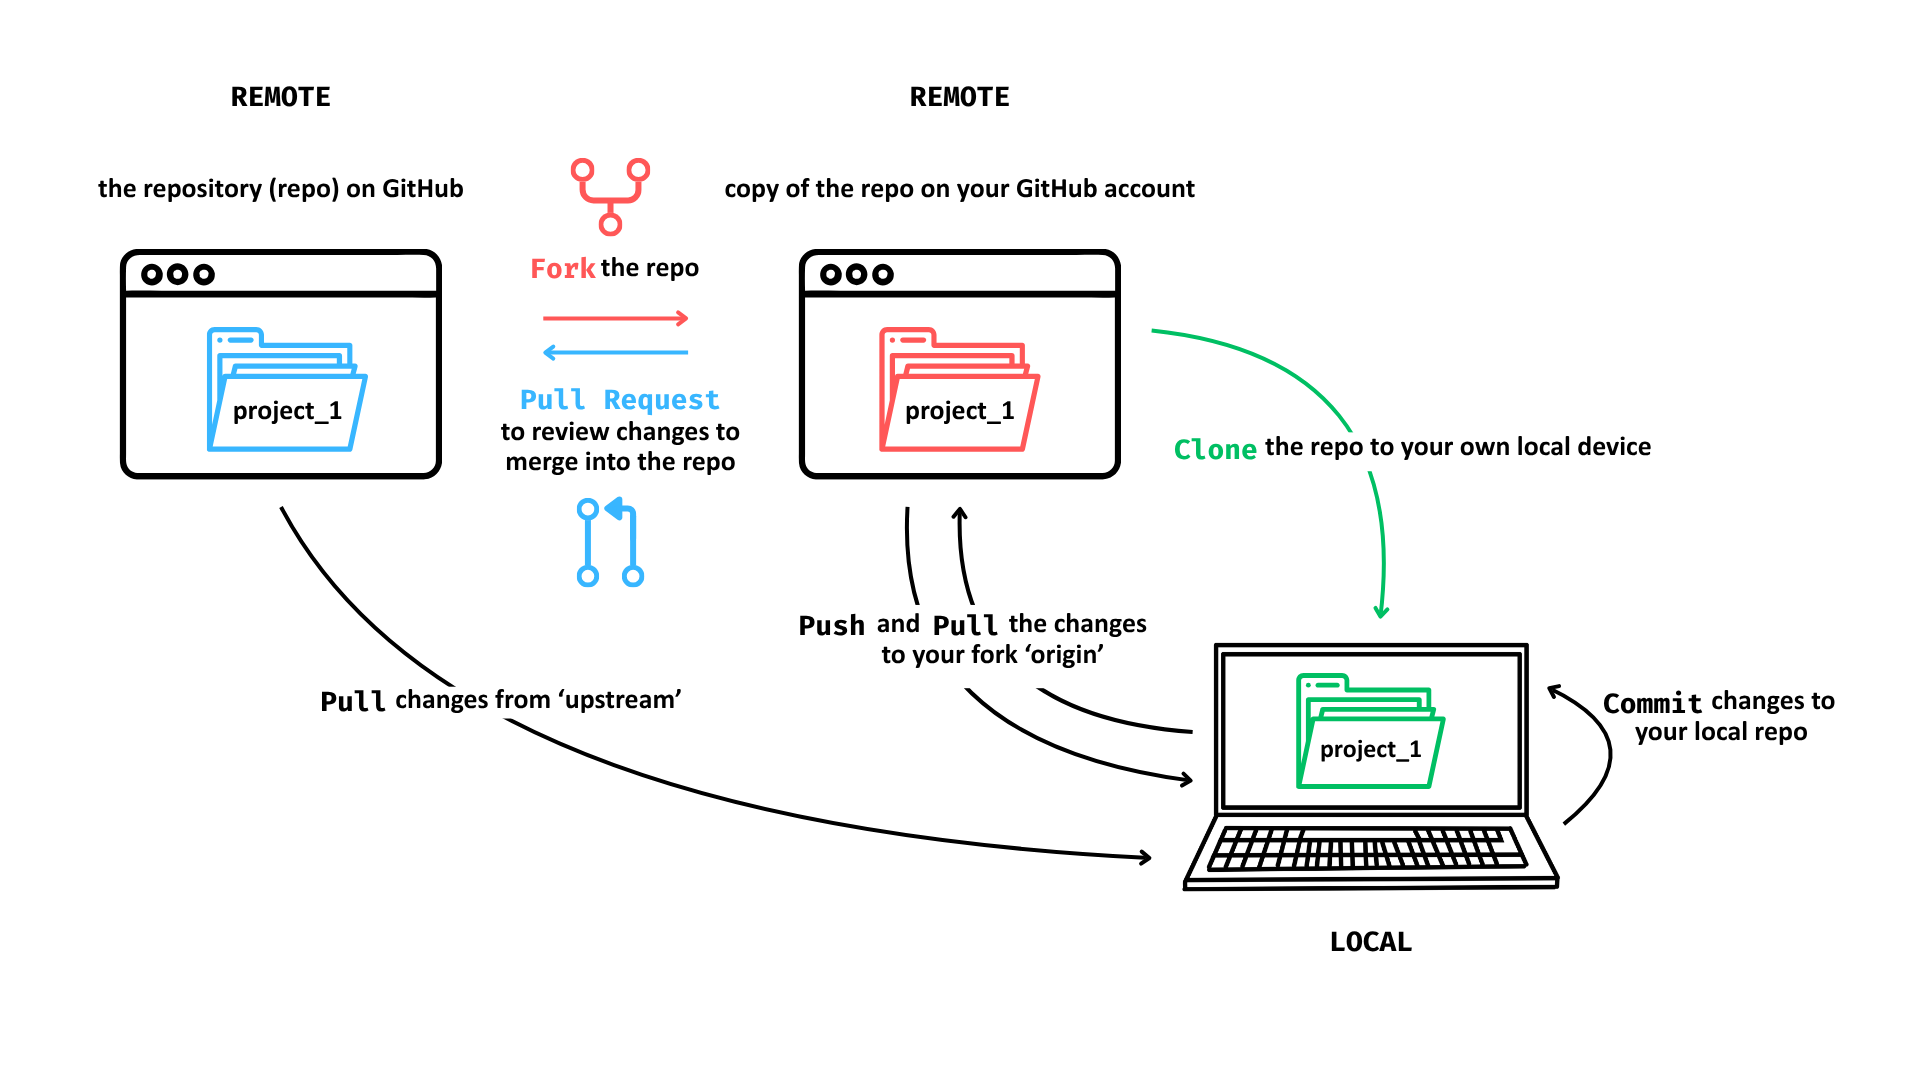
\includegraphics[keepaspectratio]{images/03_GitHub_Workflow.png}}
\end{center}

\textbf{Presenter Notes}: Here is what a typical workflow using GitHub
looks like:

\begin{itemize}
\tightlist
\item
  Start with a central repository that contains the shared project
  files.
\item
  Fork the repository to create your own copy on GitHub.
\item
  Clone your fork to your local computer so you can work offline.
\item
  Make changes locally and commit them to track your progress.
\item
  Push your commits to your fork on GitHub without affecting anyone
  else's work.
\item
  Pull updates from the main branch regularly to keep your copy up to
  date.
\item
  When your changes are ready, open a pull request so they can be
  reviewed and merged into the main branch.
\end{itemize}

\textbf{Instructor Notes}: Learners with no prior knowledge in GitHub
may not know what any of these terms mean but this is a helpful
introduction to how the different actions on GitHub come together to
create a workflow and would help learners make the connection between
them as they follow along in this session to learn them. This image will
be shown again at the end so learners can have a chance to view the
diagram with a clearer understanding of what the terms mean. \textbf{An
activity suggestion}: Have learners work in pairs or small groups to
discuss the question ``What problems does this workflow solve?'' Look at
the diagram and reflect on some of the solutions GitHub provide and see
where or what step in the workflow helps with the challenges in
collaboration (for example: cloning the repo so the copy on the local
device is still connected to the main project helps solve the issue of
disconnected collaboration.)

\begin{center}\rule{0.5\linewidth}{0.5pt}\end{center}

\subsection{Fork a repo}\label{fork-a-repo}

To \textbf{fork a repo} means to copy a collaborator's repo to your own
remote \emph{GitHub account}.

\begin{itemize}
\tightlist
\item
  Enables multiple contributors to work in parallel.
\item
  Make changes without affecting the original project.
\item
  Provides a personal workspace to test ideas.
\end{itemize}

\textbf{Presenter Notes}: Now let us go through each of the steps in the
workflow and practice them. The first step is to make your own copy of
the project repository to your GitHub account. To do this, you need to
fork the repo, which means to copy it so that you have your own version
where you can host your changes to send it with changes back to the main
repository later. How does this contribute towards collaboration? It
enables multiple contributors to work on the project at the same time.
The changes you make on your copy won't affect the original project, so
it becomes your personal workspace where you can freely test ideas
ideas.

\textbf{Instructor Notes}: This is where the practice repo you had set
up comes in. The learners will make a fork of the one you previously
forked from the OSC GitHub account.

\begin{center}\rule{0.5\linewidth}{0.5pt}\end{center}

\subsection{Practical exercise 1: Fork a
repo}\label{practical-exercise-1-fork-a-repo}

Here's a link to the main repository:

\begin{itemize}
\tightlist
\item[$\square$]
  Go to the \textbf{repository ( = ``repo'') on GitHub}:
  \href{insert\%20the\%20link\%20to\%20the\%20practice\%20reposiory\%20here}{insert
  a title of the link here}
\end{itemize}

\begin{tcolorbox}[enhanced jigsaw, colbacktitle=quarto-callout-important-color!10!white, opacityback=0, leftrule=.75mm, colback=white, opacitybacktitle=0.6, colframe=quarto-callout-important-color-frame, title=\textcolor{quarto-callout-important-color}{\faExclamation}\hspace{0.5em}{What is meant by ``\textbf{repo}'' here?}, left=2mm, titlerule=0mm, toptitle=1mm, breakable, bottomtitle=1mm, arc=.35mm, rightrule=.15mm, bottomrule=.15mm, toprule=.15mm, coltitle=black]

By \textbf{repo on GitHub} we mean one of two things: 1) the repository
your instructor created on their own remote GitHub account for you to
work on, \textbf{or} 2) an existing repo for practice e.g.,
\url{https://github.com/lmu-osc/Collaborative-RStudio-GitHub/tree/main}.
Go to the repo that is available to you \emph{now}.

\end{tcolorbox}

\textbf{Presenter Notes}: Go to the main repository of the project we
will be using for today, e,g., the repository that I provided you with
today. Click the link to be redirected to the repository on GitHub.

\textbf{Instructor Notes}: Provide learners with the name or link to
your forked repo created for this session. Replace the information in
the first line with the practice repository. Make a title for the link
(for e.g., ``Practice Repository for Collaborative Coding'') in the
square brackets and then copy and paste the url link to the practice
repository in the brackets. This way, the learners can easy navigate to
the practice repository they must then fork in the next slide.

\begin{center}\rule{0.5\linewidth}{0.5pt}\end{center}

\subsection{Practical exercise 1: Fork a
repo}\label{practical-exercise-1-fork-a-repo-1}

\begin{center}
\pandocbounded{
\includegraphics[keepaspectratio]{OS-M3-S5-GitHub-slides_files/mediabag/fork-button.png}}
\end{center}

\begin{itemize}
\tightlist
\item[$\square$]
  Click on ``\texttt{Fork}'' in the top-right toolbar
\end{itemize}

\begin{tcolorbox}[enhanced jigsaw, colbacktitle=quarto-callout-important-color!10!white, opacityback=0, leftrule=.75mm, colback=white, opacitybacktitle=0.6, colframe=quarto-callout-important-color-frame, title=\textcolor{quarto-callout-important-color}{\faExclamation}\hspace{0.5em}{Something does not look the same?}, left=2mm, titlerule=0mm, toptitle=1mm, breakable, bottomtitle=1mm, arc=.35mm, rightrule=.15mm, bottomrule=.15mm, toprule=.15mm, coltitle=black]

Note that \textbf{the screenshot may not match exactly} because it
depends which repo you \emph{forked from}: You may be forking from your
instructor's GitHub instead of from the practice repo from `lmu-osc'.

\end{tcolorbox}

\textbf{Presenter Notes}: On the repository, find the toolbar at the top
that is next to the name of the repository and click ``Fork''.

\textbf{Instructor Notes}: The `main repository' here will be the one
that you forked from the original lmu-osc tutorial and was subsequently
copied to your own remote GitHub account. In essence, your learners are
now creating a fork of your fork. This is also the first instance where
what you and your learners see on screen may not match identically with
what this example image shows.

\begin{center}\rule{0.5\linewidth}{0.5pt}\end{center}

\subsection{Practical exercise 1: Fork a
repo}\label{practical-exercise-1-fork-a-repo-2}

\begin{center}
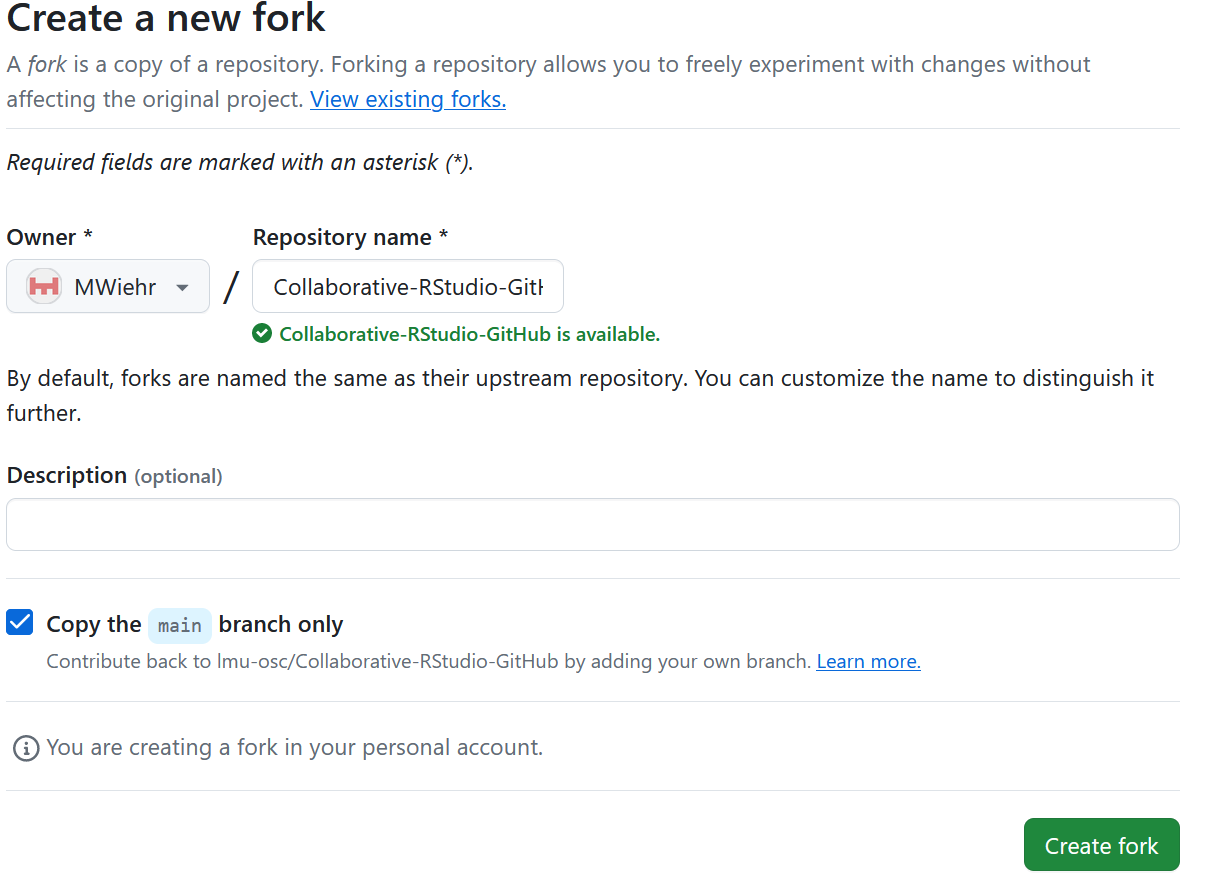
\includegraphics[width=0.7\linewidth,height=\textheight,keepaspectratio]{OS-M3-S5-GitHub-slides_files/mediabag/create-fork.png}
\end{center}

\begin{itemize}
\tightlist
\item[$\square$]
  Choose your GitHub account as the ``\texttt{owner}''
\item[$\square$]
  Click on the green ``\texttt{Create\ fork}'' button at the
  bottom-right of the screen
\end{itemize}

\textbf{Presenter Notes}: It takes you to a new page where you will
change the `owner' to your GitHub account, leave the repository name as
is and then click the green ``Create fork'' button at the bottom.

\textbf{Instructor Notes}: The only thing that should look different for
each learner is the ``Owner'' field- it should reflect each individual's
GitHub account name.

\begin{center}\rule{0.5\linewidth}{0.5pt}\end{center}

\subsection{Fork a repo}\label{fork-a-repo-1}

You will see the fork of the repository on \textbf{your} GitHub account:

\pandocbounded{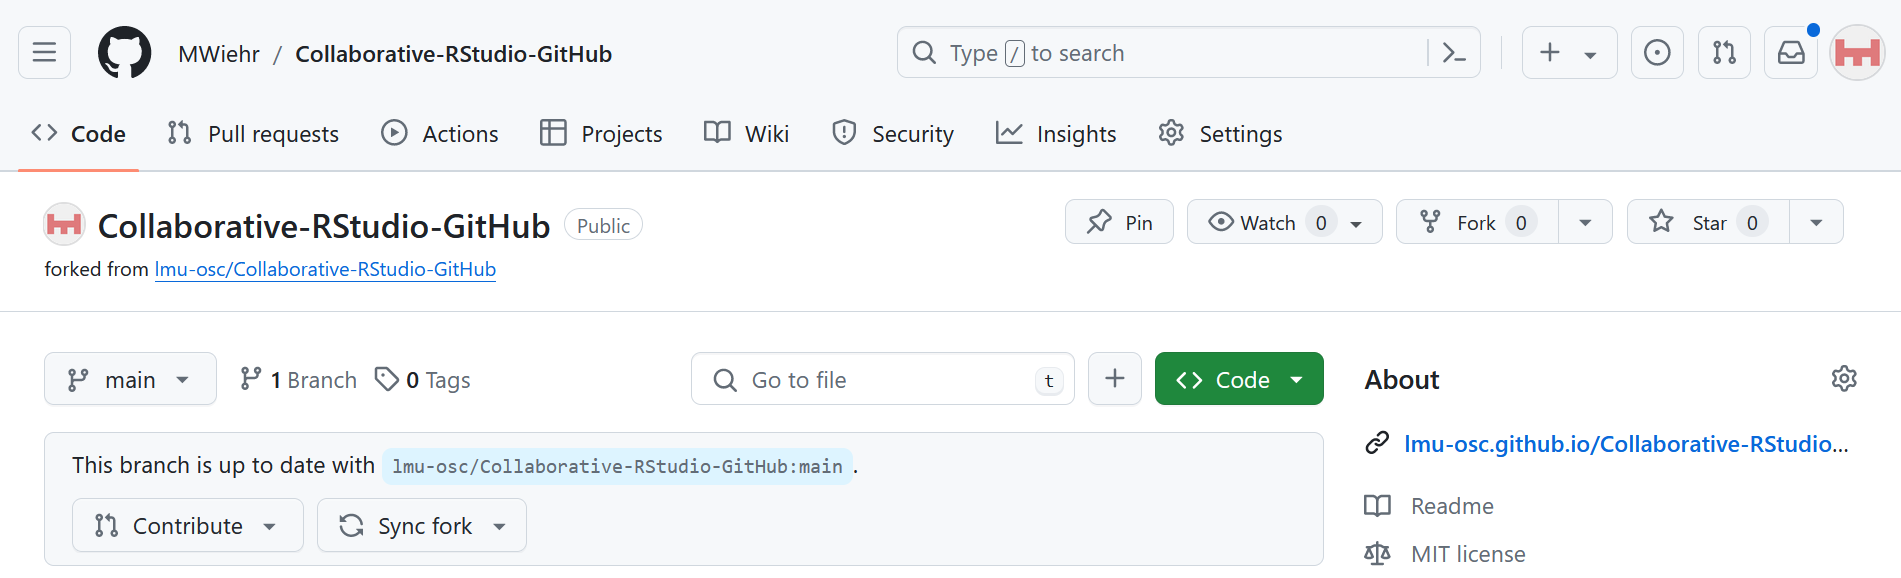
\includegraphics[keepaspectratio]{OS-M3-S5-GitHub-slides_files/mediabag/fork-process.png}}

\textbf{Presenter Notes}: When you click on the drop-down arrow next to
``Fork'' on the main repository, you will see your fork of the
repository on your GitHub account.

\begin{center}\rule{0.5\linewidth}{0.5pt}\end{center}

\subsection{Clone a repo}\label{clone-a-repo}

To \textbf{clone a repo} means to copy the project files onto your
\emph{local device}, such as your personal computer.

\begin{itemize}
\tightlist
\item
  Connects your local work directly to the team's online repository.
\item
  Makes it easy to sync updates between contributors.
\end{itemize}

\begin{tcolorbox}[enhanced jigsaw, colbacktitle=quarto-callout-important-color!10!white, opacityback=0, leftrule=.75mm, colback=white, opacitybacktitle=0.6, colframe=quarto-callout-important-color-frame, title=\textcolor{quarto-callout-important-color}{\faExclamation}\hspace{0.5em}{Important difference: Forking vs.~cloning}, left=2mm, titlerule=0mm, toptitle=1mm, breakable, bottomtitle=1mm, arc=.35mm, rightrule=.15mm, bottomrule=.15mm, toprule=.15mm, coltitle=black]

When you \textbf{fork} the repo, a copy is made on your \emph{remote
GitHub account}. When you \textbf{clone} a repo, a copy is downloaded
from GitHub onto your \emph{local device}.

\end{tcolorbox}

\textbf{Presenter Notes}: To work on your copy or version of the
project, clone it to your personal device. When you clone the repo, it
takes the project from GitHub and downloads it onto your personal device
so now you have an offline version of the project to work on. How does
this contribute towards collaboration? You can now have a copy of the
project files on your local device that's still connected to the online
repository and it makes it easy to sync updates between contributors.

\textbf{Instructor Notes}: Both forking and cloning involve making
copies of the repo but to different locations, so make this distinction
clear. If there is any confusion, you can go back to the first diagram
of the workflow to visualize the difference.

\begin{center}\rule{0.5\linewidth}{0.5pt}\end{center}

\subsection{Practical exercise 2: Clone a
repo}\label{practical-exercise-2-clone-a-repo}

\begin{center}
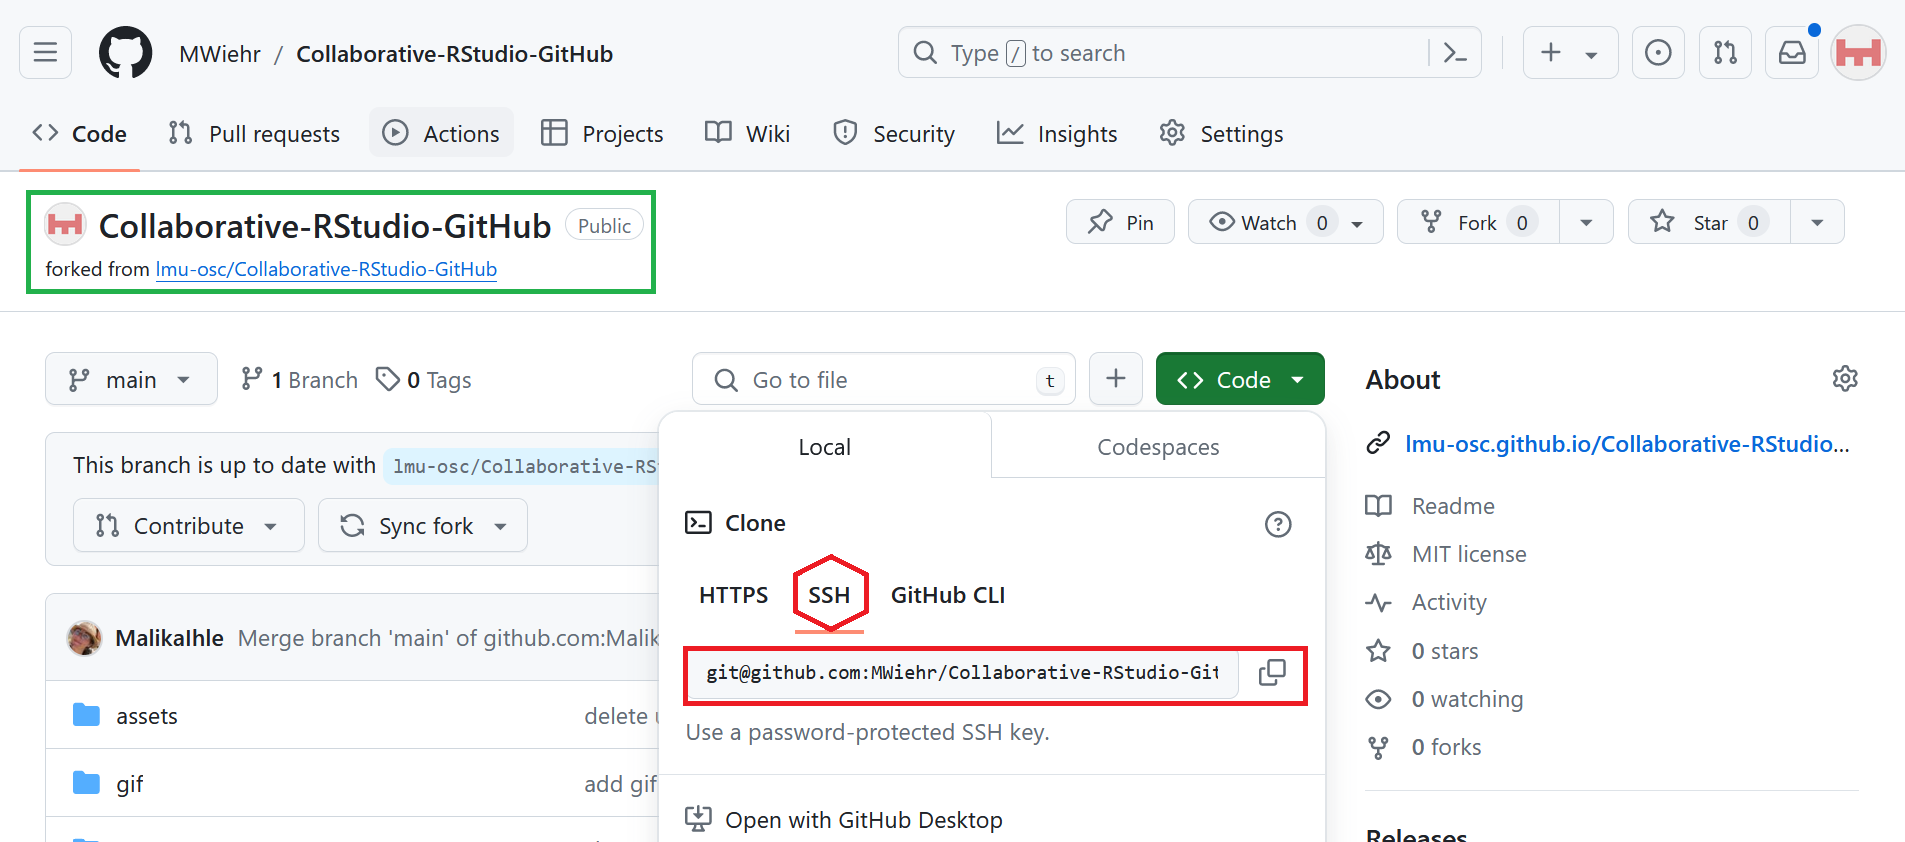
\includegraphics[width=0.6\linewidth,height=\textheight,keepaspectratio]{OS-M3-S5-GitHub-slides_files/mediabag/clone-button.png}
\end{center}

\begin{itemize}
\tightlist
\item[$\square$]
  In your fork, click on the green
  ``\texttt{\textless{}\textgreater{}\ Code}'' button
\item[$\square$]
  Click on the ``\texttt{SSH}'' tab to get the URL
\item[$\square$]
  Copy the repository's URL
\end{itemize}

\textbf{Presenter Notes}: Let us practice this using the forked
repository you just made. In your fork, find the green ``Code button''.
Once you find that, it will most likely be on the HTTPS tab, so we need
to click on the SSH tab instead and copy the URL given there.

\begin{center}\rule{0.5\linewidth}{0.5pt}\end{center}

\subsection{Practical exercise 2: Clone a
repo}\label{practical-exercise-2-clone-a-repo-1}

\begin{center}
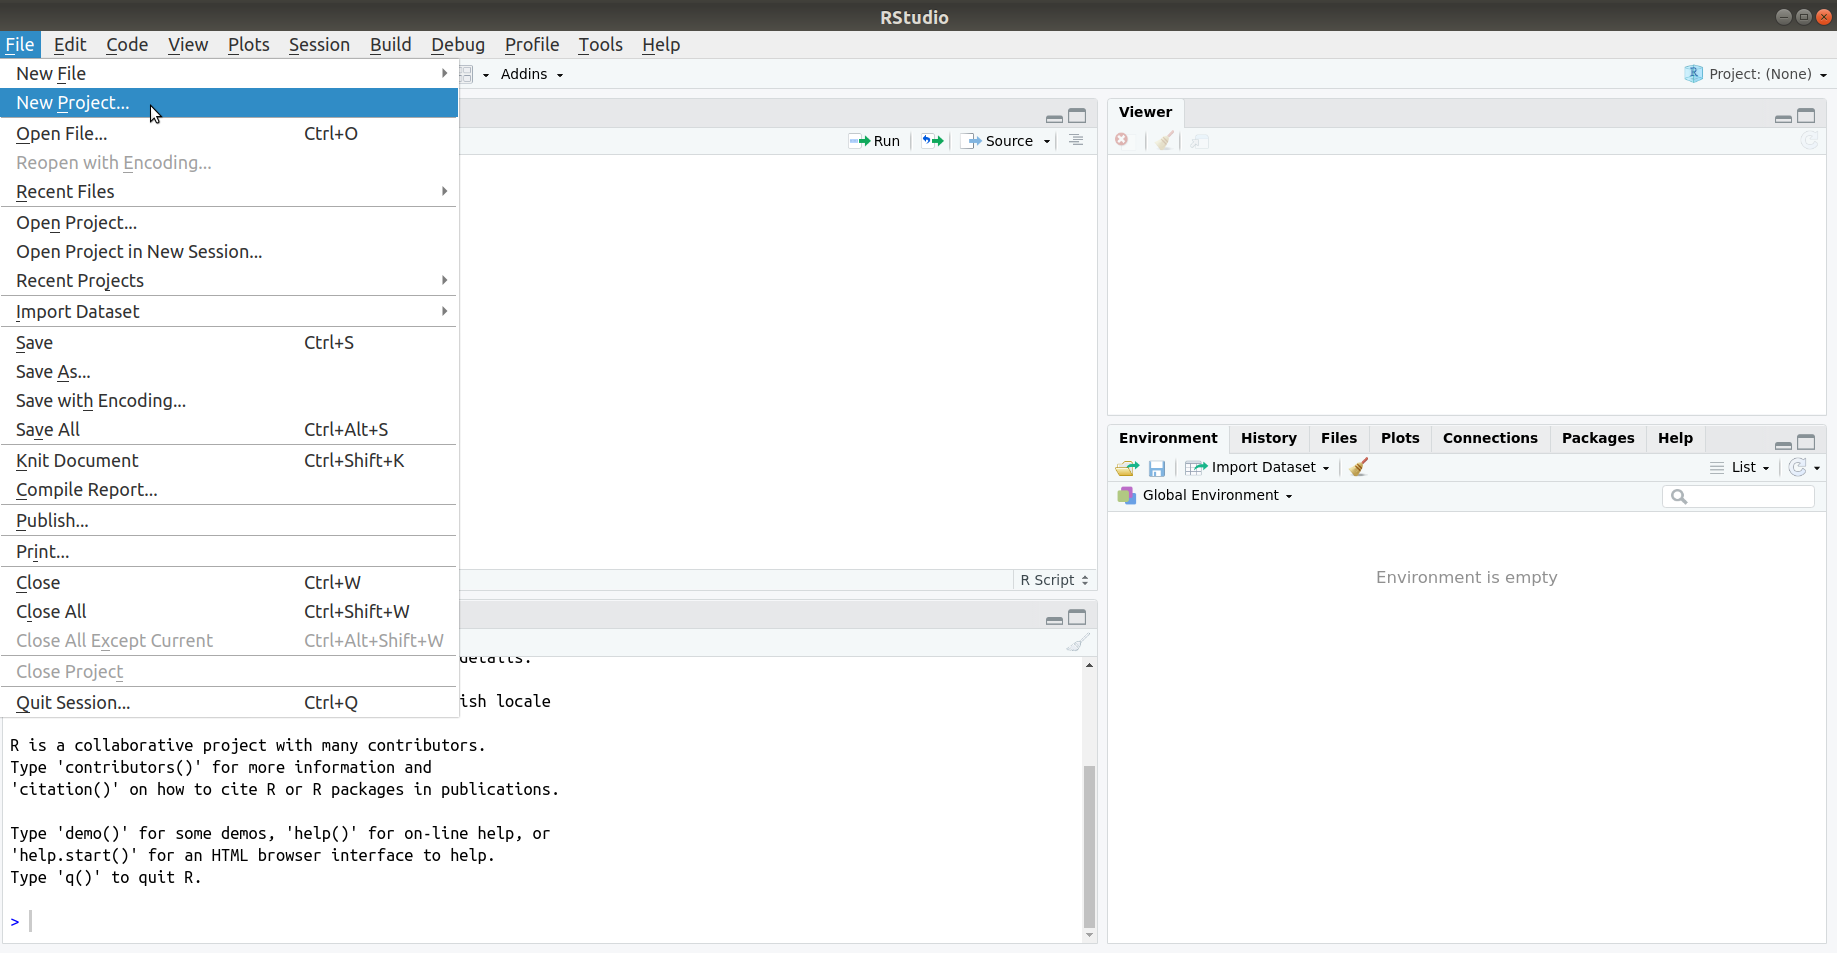
\includegraphics[width=0.7\linewidth,height=\textheight,keepaspectratio]{OS-M3-S5-GitHub-slides_files/mediabag/new-project.png}
\end{center}

\begin{itemize}
\tightlist
\item[$\square$]
  In \textbf{RStudio}, click ``\texttt{File}'' -\textgreater{}
  ``\texttt{New\ Project}'' to open a new project
\end{itemize}

\textbf{Presenter Notes}: - Now let's switch to RStudio where we can use
the built-in functions for Git. This way we can make our changes and
manage our workflow in one place. - When you clone the files, you will
put them in a new project on your device. To do this: open RStudio and
go to `File' then create a new project by selecting ``New Project''.

\textbf{Instructor Notes}: RStudio provides a simple point-and-click
interface to perform some of the actions in the GitHub workflow,
however, there are other ways to communicate with GitHub using your
local device.

\begin{center}\rule{0.5\linewidth}{0.5pt}\end{center}

\subsection{Practical exercise 2: Clone a
repo}\label{practical-exercise-2-clone-a-repo-2}

\begin{center}
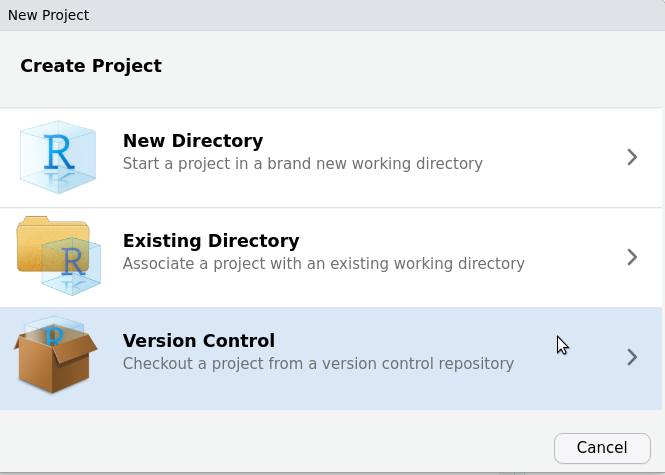
\includegraphics[width=0.8\linewidth,height=\textheight,keepaspectratio]{OS-M3-S5-GitHub-slides_files/mediabag/version-control-proj.png}
\end{center}

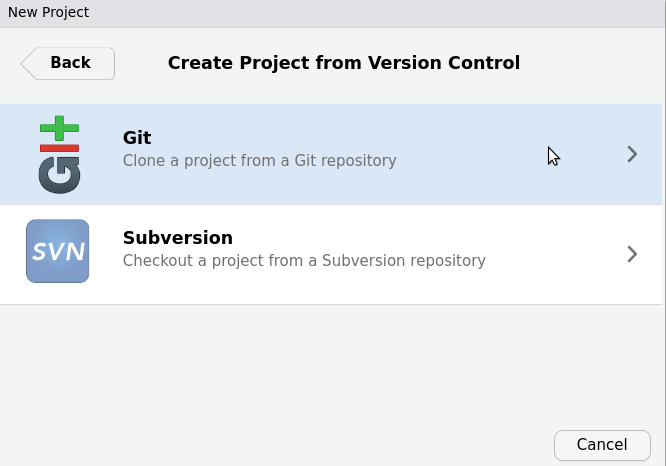
\includegraphics[width=0.8\linewidth,height=\textheight,keepaspectratio]{OS-M3-S5-GitHub-slides_files/mediabag/git-project.png}

\begin{itemize}
\tightlist
\item[$\square$]
  Select the ``\texttt{Version\ Control}'' option
\end{itemize}

\begin{itemize}
\tightlist
\item[$\square$]
  Select the ``\texttt{Git}'' option
\end{itemize}

\textbf{Presenter Notes}: We need to select ``Version Control'' to
connect RStudio directly to the GitHub repository and work with
version-tracked code. Then, we select ``Git'' to clone the project
directly from the GitHub repository.

\textbf{Instructor Notes}: The ``Git'' option appears if Git is
correctly installed on your device. If it does not appear, check if Git
has been installed and restart RStudio.

\begin{center}\rule{0.5\linewidth}{0.5pt}\end{center}

\subsection{Practical exercise 2: Clone a
repo}\label{practical-exercise-2-clone-a-repo-3}

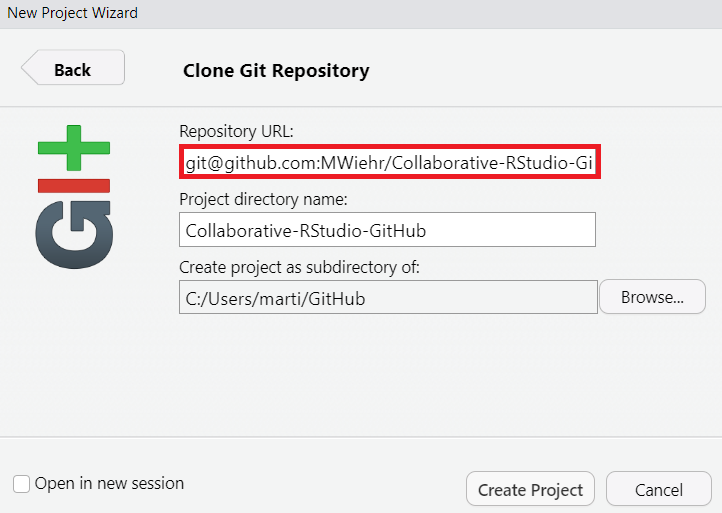
\includegraphics[width=0.9\linewidth,height=\textheight,keepaspectratio]{OS-M3-S5-GitHub-slides_files/mediabag/paste-url.png}

\begin{itemize}
\tightlist
\item[$\square$]
  Paste the URL of the GitHub repository under
  ``\texttt{Repository\ URL:}''
\item[$\square$]
  Click ``\texttt{Create\ Project}''
\item[$\square$]
  Click ``\texttt{Browse...}'' to place the project in a new folder on
  your device
\end{itemize}

\begin{tcolorbox}[enhanced jigsaw, colbacktitle=quarto-callout-important-color!10!white, opacityback=0, leftrule=.75mm, colback=white, opacitybacktitle=0.6, colframe=quarto-callout-important-color-frame, title=\textcolor{quarto-callout-important-color}{\faExclamation}\hspace{0.5em}{Placing this project in a new folder}, left=2mm, titlerule=0mm, toptitle=1mm, breakable, bottomtitle=1mm, arc=.35mm, rightrule=.15mm, bottomrule=.15mm, toprule=.15mm, coltitle=black]

First, make a new folder on your device. Then, you can change the path
under ``\texttt{Create\ project\ as\ subdirectroy\ of:}'' to place this
Git repository in that new folder. We are making a new folder because it
is advisable that each folder has its own Git database.

\end{tcolorbox}

\textbf{Presenter Notes}: Remember the URL we copied from the SSH tab?
Now we need to paste it under ``Repository URL''. If you've created a
folder with a Git database for a previous lesson, make a new one for
this. When you make a new folder, click ``Browse\ldots{}'' and select
that folder. Each folder should have it's own Git database. Next, when
you hit ``Create Project'', you'll need to enter your password.

\textbf{Instructor Notes}: If learners are confused as to which password
is required: it is the password for their individual GitHub accounts.

\begin{center}\rule{0.5\linewidth}{0.5pt}\end{center}

\subsection{Clone a repo}\label{clone-a-repo-1}

\begin{center}
\pandocbounded{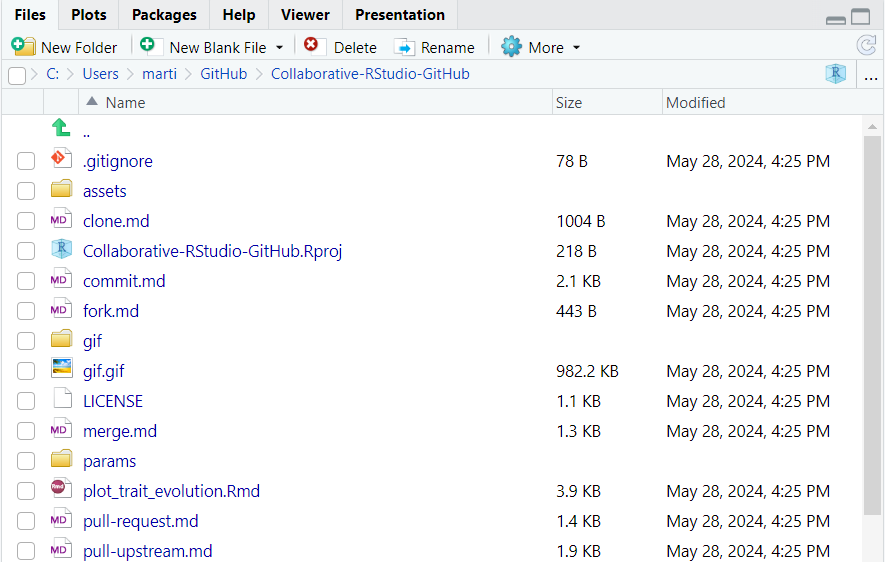
\includegraphics[keepaspectratio]{OS-M3-S5-GitHub-slides_files/mediabag/files-tab.png}}
\end{center}

Now, when you click on the ``\texttt{Files}'' tab in \textbf{RStudio},
you should see all the files from the main repository.

\textbf{Presenter Notes}: And that's it! You should now have the files
from the main repository on your local device. Check this by clicking on
the ``Files'' tab in RStudio and check that all the files from the main
repository are now appearing. Compare what you have on your RStudio
project to what is in your fork on GitHub.

\textbf{Instructor Notes}: It would be helpful at this stage to point
out the ``params'' sub-folder as one of the files here in the cloned
repository. This is the sub-folder containing the R file that learners
will need to copy in the next exercise.

\begin{center}\rule{0.5\linewidth}{0.5pt}\end{center}

\subsection{Commit to a project}\label{commit-to-a-project}

To \textbf{commit to a project} means to save the file with the changes
you made locally in your version control system.

\begin{itemize}
\tightlist
\item
  Records progress in small and trackable steps
\item
  Lets others see exactly what was changed
\item
  Makes it possible to revert or review changes if there are bugs
\end{itemize}

\begin{tcolorbox}[enhanced jigsaw, colbacktitle=quarto-callout-tip-color!10!white, opacityback=0, leftrule=.75mm, colback=white, opacitybacktitle=0.6, colframe=quarto-callout-tip-color-frame, title=\textcolor{quarto-callout-tip-color}{\faLightbulb}\hspace{0.5em}{Avoiding merge conflicts}, left=2mm, titlerule=0mm, toptitle=1mm, breakable, bottomtitle=1mm, arc=.35mm, rightrule=.15mm, bottomrule=.15mm, toprule=.15mm, coltitle=black]

\textbf{Merge conflicts} happen when Git cannot automatically combine
changes because the same part of a file was edited differently by two
collaborators. Frequent commits help with resolving conflicts because
they create clear checkpoints in your project's history. GitHub also
offers
\href{https://docs.github.com/en/issues/tracking-your-work-with-issues/learning-about-issues/about-issues}{GitHub
issues} as a communication tool to resolve conflicts.

\end{tcolorbox}

\textbf{Presenter Notes}: A commit is like taking a snapshot of your
project after you make changes. Each commit records what was changed,
when, and by whom. You usually include a short message describing the
update, for example, ``Updated code for analysis,'' and saves it in
Git's version history. How does this contribute towards collaboration?
Frequent commits records the progress of each contributor in small,
trackable steps. It let's others see what changes had been made.
Frequent commits also make it possible to review changes if something
breaks because now you can go back, review changes, and isolate problems
to fix it.

\begin{center}\rule{0.5\linewidth}{0.5pt}\end{center}

\subsection{Practical exercise 3:
Commit}\label{practical-exercise-3-commit}

Before you \textbf{commit to a project}, you need to make some changes
to the project.

\begin{center}
\pandocbounded{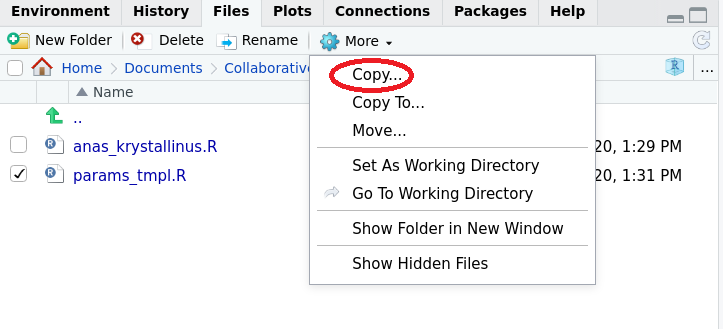
\includegraphics[keepaspectratio]{OS-M3-S5-GitHub-slides_files/mediabag/copy-params_tmpl.png}}
\end{center}

\begin{itemize}
\tightlist
\item[$\square$]
  Go into the ``\texttt{params}'' sub-folder by clicking it in
  \textbf{RStudio}
\item[$\square$]
  Select the ``\texttt{params\_templ.R}'' file
\item[$\square$]
  Click ``\texttt{More}'' then ``\texttt{Copy...}'' to make a copy of
  this file
\end{itemize}

\textbf{Presenter Notes}: We are still in RStudio. In the `Files' tab,
find the `params' sub-folder and open it. Now within this sub-folder,
find an R file called `params\_templ' and click the tickbox next to it
to select it. This is what where we will be making our changes to the
project. Then click on the drop-down arrow by ``More'' and click
``Copy''.

\textbf{Instructor Notes}: Copying the file and then editing the copied
file is specific to this practice exercise. You do not always need to
copy the file to then make changes to it, a project can require a
contributor to make changes to the file directly. It depends on the
project.

\begin{center}\rule{0.5\linewidth}{0.5pt}\end{center}

\subsection{Practical exercise 3:
Commit}\label{practical-exercise-3-commit-1}

\begin{itemize}
\tightlist
\item[$\square$]
  Enter a name for your copied file like in the example below:
\end{itemize}

\begin{itemize}
\tightlist
\item[$\square$]
  Open your copy of the file to make your changes (in this case, you
  will be making a new parameter)
\end{itemize}

\textbf{Presenter Notes}: You'll be prompted to give the copied file a
name/title, use something identifiable like including your first name.

\begin{center}\rule{0.5\linewidth}{0.5pt}\end{center}

\subsection{Practical exercise 3:
Commit}\label{practical-exercise-3-commit-2}

\begin{center}
\pandocbounded{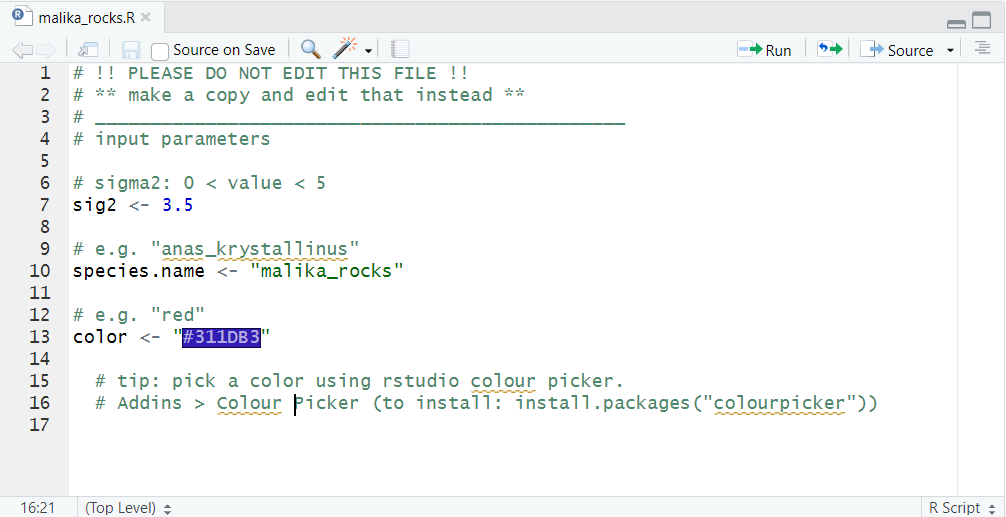
\includegraphics[keepaspectratio]{OS-M3-S5-GitHub-slides_files/mediabag/edit-file.png}}
\end{center}

\begin{itemize}
\tightlist
\item[$\square$]
  For \texttt{sig2}: type in a numeric value greater than 0 but smaller
  than 5 with NO quotation marks around it.
\item[$\square$]
  For \texttt{species.name}: type a character string with quotation
  marks (for example, ``anas\_krystallinus''). Try making a species name
  out of your name!
\item[$\square$]
  For \texttt{color}: type the hex code of a color with quotation marks
  (for example, the color red is ``\#FFFFFF'').
\end{itemize}

\textbf{Presenter Notes}: In this exercise, each person will edit their
own parameter file to practice making a commit. Update these three
values: a numeric for ``sig2'', a character name for ``species.name'',
and a hex color code for ``color''. You can install the package
``colourpicker'' which would create an Addin called ``Colour Picker'' to
help find a hex code for a desired color. The ``Addins'' drop-down menu
is found on a toolbar at the top of the RStudio workspace.

\textbf{Instructor Notes}: Make sure learners do NOT put additional
information (more than what's required) as this can result in the code
breaking.

\begin{center}\rule{0.5\linewidth}{0.5pt}\end{center}

\subsection{Practical exercise 3:
Commit}\label{practical-exercise-3-commit-3}

\begin{itemize}
\tightlist
\item[$\square$]
  Save your file by going to the top toolbar and clicking
  ``\texttt{File}'' -\textgreater{} then ``\texttt{Save}''
\end{itemize}

\begin{center}
\pandocbounded{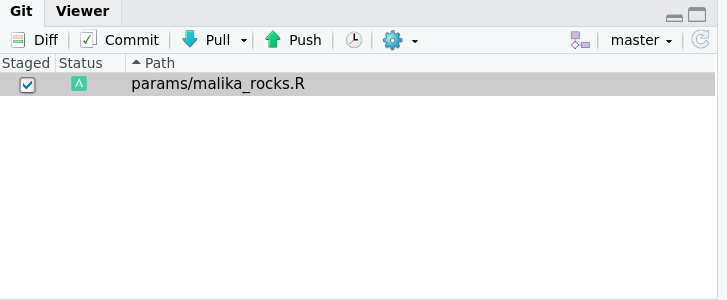
\includegraphics[keepaspectratio]{OS-M3-S5-GitHub-slides_files/mediabag/stage.png}}
\end{center}

\begin{itemize}
\tightlist
\item[$\square$]
  In the ``\texttt{Git}'' tab, tick the checkbox next to \emph{your
  copied file}. This will \textbf{stage} your file
\item[$\square$]
  Click ``\texttt{Commit}''
\end{itemize}

\textbf{Presenter Notes}: After this, save the file as normal by going
to ``File'' and then clicking ``Save''. In the Git tab on RStudio, tick
the checkbox next to your copied file under the ``Staged'' column.
Staging a commit means you're selecting which specific changes you want
to include in your next commit. Then click the ``Commit'' button.

\begin{center}\rule{0.5\linewidth}{0.5pt}\end{center}

\subsection{Practical exercise 3:
Commit}\label{practical-exercise-3-commit-4}

\begin{center}
\pandocbounded{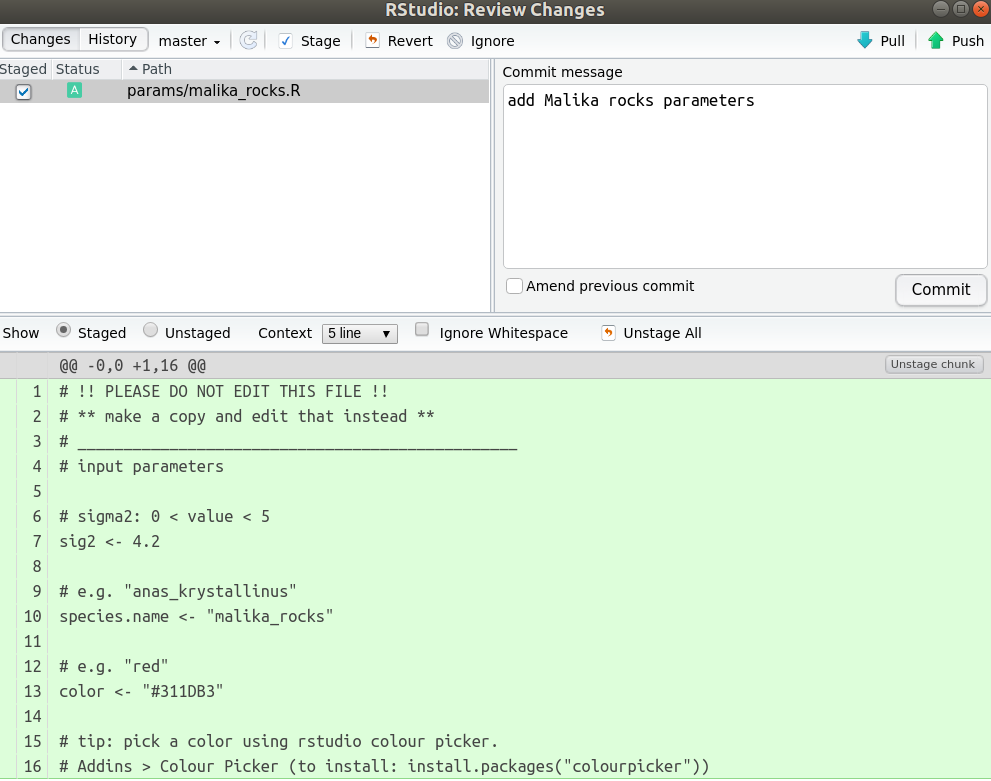
\includegraphics[keepaspectratio]{OS-M3-S5-GitHub-slides_files/mediabag/commit.png}}
\end{center}

\begin{itemize}
\tightlist
\item[$\square$]
  Add a comment in the ``\texttt{Commit\ message}'' box briefly
  describing the changes you made (for example: ``add Malika rocks
  parameters'')
\item[$\square$]
  Click ``\texttt{Commit}'' under the ``\texttt{Commit\ message}''
  textbox
\end{itemize}

\textbf{Presenter Notes}: You should leave a message to accompany your
commit. This is like describing the changes you made to make your
commits more informative. For example, just state what you added to the
file. Then, Click the ``Commit'' button.

\textbf{Instructor Notes}: You can remind learners that this does not
mean their changes will show up on GitHub, that requires an additional
step. But this does mean their activity and changes were recorded in the
project history.

\begin{center}\rule{0.5\linewidth}{0.5pt}\end{center}

\subsection{You made a contribution!}\label{you-made-a-contribution}

Great, now you have made changes! You added a file with your parameters
on a shared project and committed it. Let's take a minute
(\emph{literally}) and recap what you did to achieve that.

\textbf{Activity: one-minute paper!}

\begin{itemize}
\tightlist
\item
  You have 60 seconds to write down \textbf{what steps you took} to
  collaborate on this project \emph{so far}.
\item
  Think of the \textbf{names of the actions}, in which \textbf{order}
  you did them, and \textbf{how can this be beneficial} to you as a
  collaborator.
\end{itemize}

\textbf{Presenter Notes}: You have successfully made a contribution by
copying a file and making some changes to it in the shared project. This
is how collaboration on GitHub happens - by each contributor having
their own copies of the project and making their individual changes.
Before we go further, let's take a minute to recap what steps we took to
get here with this activity. You have 60 seconds to write down these
steps. Think of the names of the actions, in which order you did them,
and how can this be beneficial to you as a collaborator.

\textbf{Instructor Notes}: This one-minute paper activity is to give the
instructor an idea of how the learners are progressing with the steps of
collaborative coding so far and if they are understanding how the steps
fit into a workflow using GitHub. It also doubly acts as a way to
reinforce the concepts discussed in this session. If you want to make
the activity a bit easier, you can provide them with the terms:
\textbf{repo, fork, clone, commit}.

\begin{center}\rule{0.5\linewidth}{0.5pt}\end{center}

\subsection{Push changes}\label{push-changes}

To \textbf{push changes} means to upload your local commits from your
local computer to the remote repository on GitHub.

\begin{itemize}
\tightlist
\item
  Keeps the online version of the project up to date.
\item
  Makes your work visible to all contributors in real time.
\item
  Enables others to pull your latest edits and build on them.
\end{itemize}

\textbf{Presenter Notes}: The next step after making your changes and
committing them is to push the changes you made from your local device
onto the remote forked repository that is on your GitHub account. How
does this contribute towards collaboration? It keeps the online version
of the project up to date with all the changes made and makes it visible
to all the contributors. It also enables others working on the project
to take your edits and build on them.

\begin{center}\rule{0.5\linewidth}{0.5pt}\end{center}

\subsection{Practical exercise 4: Push}\label{practical-exercise-4-push}

\begin{center}
\pandocbounded{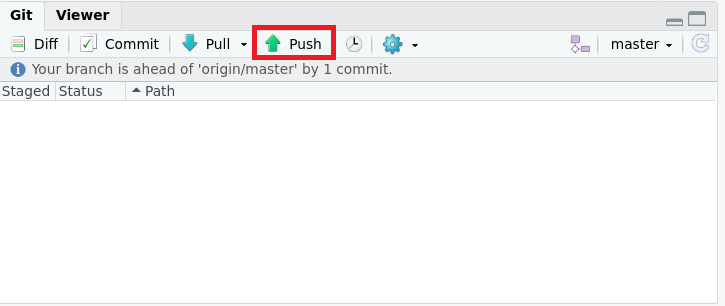
\includegraphics[keepaspectratio]{OS-M3-S5-GitHub-slides_files/mediabag/push-rstudio.png}}
\end{center}

\begin{itemize}
\tightlist
\item[$\square$]
  In the \texttt{Git} tab, click ``\texttt{Push}'' to send your changes
  to GitHub
\item[$\square$]
  Enter your password when prompted
\end{itemize}

\textbf{Presenter Notes}: The changes you made are just on your local
device and committing it means you just recorded it in the project
history. But it is not et on your remote fork on GitHub. To send the
changes you just made to the file on your local device to your online
fork on GitHub, you need to click the ``Push'' button in the Git tab.
You'll then need to enter your password again.

\begin{center}\rule{0.5\linewidth}{0.5pt}\end{center}

\subsection{Push changes}\label{push-changes-1}

If you successfully pushed your changes, you would see a pop up box like
the one below:

\begin{center}
\pandocbounded{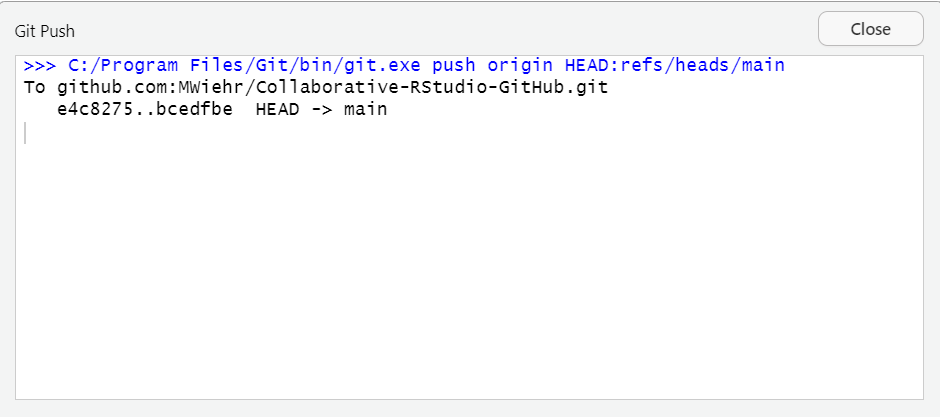
\includegraphics[keepaspectratio]{OS-M3-S5-GitHub-slides_files/mediabag/push-github.png}}
\end{center}

\textbf{Presenter Notes}: If all went well, you will see a pop up box
with a message like this one to let you know the changes were
successfully pushed to the remote repository. An additional way to make
sure your changes were pushed, refresh your GitHub repository webpage
and check to see if the file you copied is now appearing. The commit
message should also appear next to it on GitHub.

\begin{center}\rule{0.5\linewidth}{0.5pt}\end{center}

\subsection{Push changes}\label{push-changes-2}

\begin{tcolorbox}[enhanced jigsaw, colbacktitle=quarto-callout-important-color!10!white, opacityback=0, leftrule=.75mm, colback=white, opacitybacktitle=0.6, colframe=quarto-callout-important-color-frame, title=\textcolor{quarto-callout-important-color}{\faExclamation}\hspace{0.5em}{Important step: refresh the page}, left=2mm, titlerule=0mm, toptitle=1mm, breakable, bottomtitle=1mm, arc=.35mm, rightrule=.15mm, bottomrule=.15mm, toprule=.15mm, coltitle=black]

Refresh the page of your forked repository on GitHub and you should see
your new file with the commit message next to it. \textbf{Refreshing the
page} is an important step to update your forked repository with the new
file you added.

\end{tcolorbox}

\textbf{Presenter Notes}: Now go back to your forked repository on
GitHub and refresh the page. This is an important step to confirm that
the file together with the commit message are appearing and to update
your fork with the changes you made.

\textbf{Instructor Notes}: If a learner does not refresh the page, this
can cause problems during when merging. If they do not refresh the page
and simply make a pull request, an empty `params\_tmpl.R' file comes up
when the owner views the request.

\begin{center}\rule{0.5\linewidth}{0.5pt}\end{center}

\subsection{Pre-break quiz}\label{pre-break-quiz}

\begin{center}
\pandocbounded{
\includegraphics[keepaspectratio]{images/00_Particify_Survey_Rooms.png}}
\end{center}

\begin{tcolorbox}[enhanced jigsaw, colbacktitle=quarto-callout-note-color!10!white, opacityback=0, leftrule=.75mm, colback=white, opacitybacktitle=0.6, colframe=quarto-callout-note-color-frame, title=\textcolor{quarto-callout-note-color}{\faInfo}\hspace{0.5em}{Pre-break quiz}, left=2mm, titlerule=0mm, toptitle=1mm, breakable, bottomtitle=1mm, arc=.35mm, rightrule=.15mm, bottomrule=.15mm, toprule=.15mm, coltitle=black]

Please complete survey labeled ``OS-M3-S5-GitHub-prebreak\_quiz''.

\end{tcolorbox}

\textbf{Presenter Notes}: Before the break, let's take a moment to
review the things we covered in the first part of this lesson. Scan the
QR code again and find the quiz titled
``Os-M3-S5-Github-prebreak\_quiz''. This quiz has a few simple recap
questions about what we've learned so far about using GitHub for
collaboration on projects. The goal isn't to test you, but to help you
reflect on what you've learned and to see if anything needs a bit more
clarification.

\textbf{Instructor Notes}: It's important to have an idea of these key
terms because they will reappear many times throughout the rest of this
lesson. - Aim: This pre-break survey serves to examine learners' current
understanding of key concepts of the submodule. - Use free survey
software such as or other survey software (particify, formR) to
establish the following questions (shown on separate slides)

\begin{center}\rule{0.5\linewidth}{0.5pt}\end{center}

\textbf{What is GitHub mainly used for by a team working on the same
project?}

\begin{enumerate}
\def\labelenumi{\alph{enumi}.}
\item
  Editing photos online
\item
  Hosting and collaborating on code or research projects
\item
  Sending emails and important messages to team members
\item
  Backing up personal files only
\end{enumerate}

\textbf{Instructor Notes}: The correct answer is b.

\begin{center}\rule{0.5\linewidth}{0.5pt}\end{center}

\textbf{On GitHub, why would you fork a repository?}

\begin{enumerate}
\def\labelenumi{\alph{enumi}.}
\item
  To delete the original repository and start a new one
\item
  To download a copy of the remote repository to your local computer
\item
  To create your own remote copy of someone else's repository on GitHub
\item
  To merge your work into the main branch and have everyone's work in
  one folder
\end{enumerate}

\textbf{Instructor Notes}: The correct answer is c.

\begin{center}\rule{0.5\linewidth}{0.5pt}\end{center}

\textbf{What does it mean to clone a repository?}

\begin{enumerate}
\def\labelenumi{\alph{enumi}.}
\item
  You download the repository from GitHub to your local device
\item
  You create a backup of your GitHub account
\item
  You make your repository private
\item
  You copy code into a new file then upload it to GitHub
\end{enumerate}

\textbf{Instructor Notes}: The correct answer is a.

\begin{center}\rule{0.5\linewidth}{0.5pt}\end{center}

\textbf{When you make changes to a file then commit it, what happens?}

\begin{enumerate}
\def\labelenumi{\alph{enumi}.}
\item
  It deletes all previous versions of your file
\item
  It sends your work directly to the main repository
\item
  It saves your changes locally (on your device)
\item
  It approves changes made by other collaborators
\end{enumerate}

\textbf{Instructor Notes}: The correct answer is c.

\begin{center}\rule{0.5\linewidth}{0.5pt}\end{center}

\textbf{After I made changes and committed it, why would I then push the
changes?}

\begin{enumerate}
\def\labelenumi{\alph{enumi}.}
\item
  To create a new repository
\item
  To incorporate my changes into the files of the main repository
\item
  To notify my teammates that I made changes
\item
  To upload the work I saved locally to GitHub
\end{enumerate}

\textbf{Instructor Notes}: The correct answer is d.

\begin{center}\rule{0.5\linewidth}{0.5pt}\end{center}

\section{Break! 15 minutes}\label{break-15-minutes}

\begin{center}\rule{0.5\linewidth}{0.5pt}\end{center}

\subsection{Post-break quiz
discussion}\label{post-break-quiz-discussion}

What do we see in the results?

\textbf{Presenter Notes}: Let's discuss the survey answers and clarify
any questions before moving on to the next section.

\textbf{Instructor Notes} - Aim: To clarify concepts and aspects that
are not yet understood - Highlight specific answers given during the
survey - Also, use this time to clarify any confusions or questions on
specific topics learners may have from the first part of the session.

\begin{center}\rule{0.5\linewidth}{0.5pt}\end{center}

\subsection{Pull request}\label{pull-request}

To make a \textbf{pull request} means asking the repository's owner to
review the changes you made (from your fork or branch) and merge them
into the main repository on GitHub.

\begin{itemize}
\tightlist
\item
  Creates a space for discussion and code review before incorporating
  changes.
\item
  Encourages feedback and peer learning.
\item
  Maintains project quality and consistency.
\end{itemize}

\textbf{Presenter Notes}: After pushing your changes to the remote
repository, it is just on your forked copy for now and not in the main
repository that has the original project files. You then need to make a
\textbf{pull request}. This is a request on GitHub for the owner of the
main repository to review your changes and then incorporate or merge
them into the main repository. This can either add to or change the
original project files. How does this contribute towards collaboration?
The changes can be reviewed and checked for error before making it a
part of the main project. This allows for feedback, peer learning, and
maintains levels of quality and consistency across the project files.

\begin{center}\rule{0.5\linewidth}{0.5pt}\end{center}

\subsection{Practical exercise 5: Pull
request}\label{practical-exercise-5-pull-request}

\pandocbounded{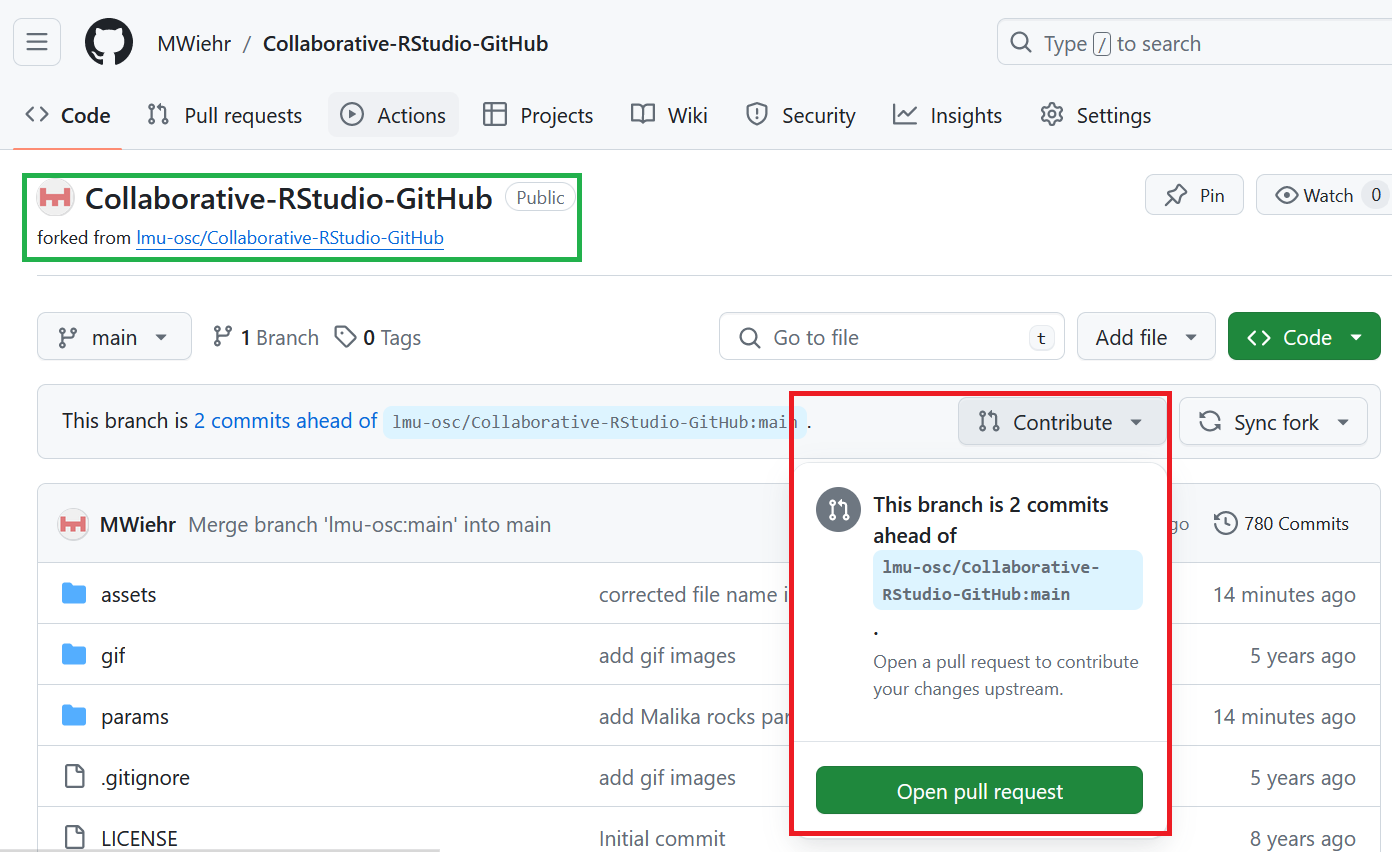
\includegraphics[keepaspectratio]{OS-M3-S5-GitHub-slides_files/mediabag/pull-request-button.png}}

\begin{itemize}
\tightlist
\item[$\square$]
  On your forked \textbf{GitHub repository}, click on
  ``\texttt{Contribute}''
\item[$\square$]
  Click on the green ``\texttt{Open\ pull\ request}'' button
\end{itemize}

\textbf{Presenter Notes}: Now we are working in the remote repository on
GitHub. In your fork, click on ``Contribute'' and then the green ``Open
pull request'' button.

\begin{center}\rule{0.5\linewidth}{0.5pt}\end{center}

\subsection{Practical exercise 5: Pull
request}\label{practical-exercise-5-pull-request-1}

\begin{center}
\pandocbounded{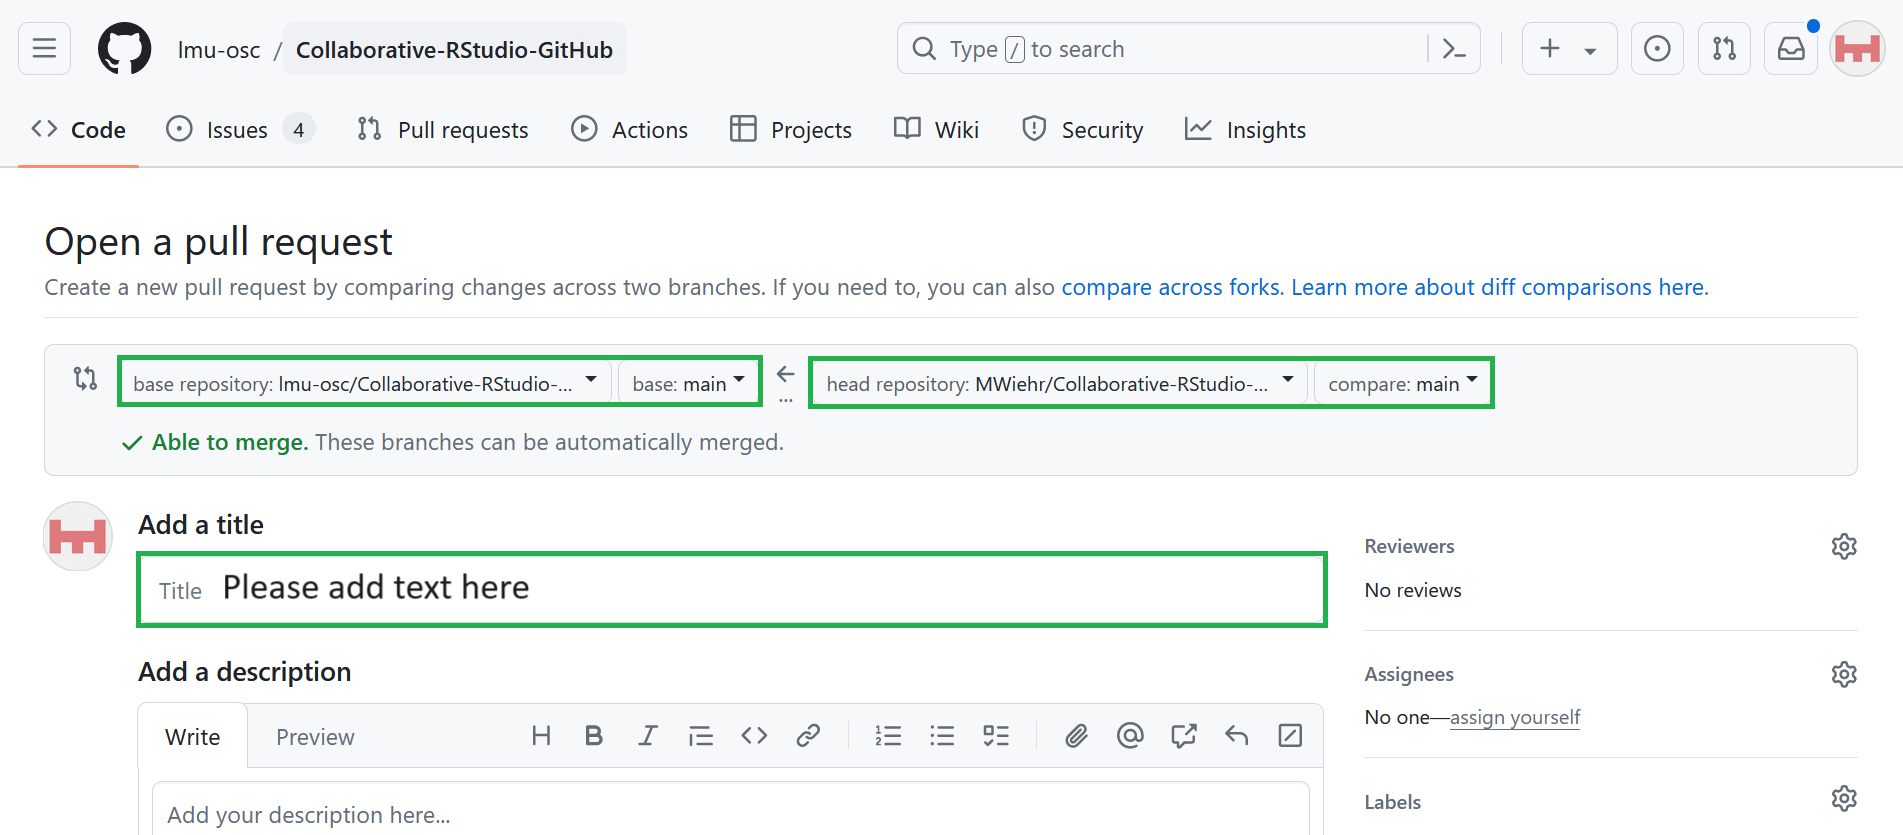
\includegraphics[keepaspectratio]{OS-M3-S5-GitHub-slides_files/mediabag/create-pull-request.png}}
\end{center}

\begin{itemize}
\tightlist
\item[$\square$]
  Ensure the \emph{base repository} is the main repository and the
  \emph{head repository} is your fork
\item[$\square$]
  Ensure your requested merge does not create any conflict (you will see
  a green ``\texttt{✓\ Able\ to\ merge}'')
\end{itemize}

\textbf{Presenter Notes}: Check the settings to ensure the ``base
repository'' is the main repository that you initially forked and the
``head repository'' is your forked repository. You should see a message
in green saying ``Able to merge'' and this means that the request to
merge does not create any conflict.

\textbf{Instructor Notes}: The `base repository' should automatically be
the one the learners forked (the main repository used in this session),
but it's important to double-check it as it will, again, not match
identically with what's shown in the example image (because you are not
using the lmu-osc original repo for this activity).

\begin{center}\rule{0.5\linewidth}{0.5pt}\end{center}

\subsection{Practical exercise 5: Pull
request}\label{practical-exercise-5-pull-request-2}

\begin{itemize}
\tightlist
\item[$\square$]
  Add a title and a message describing your contributions/changes made
\item[$\square$]
  Click ``\texttt{Create\ pull\ request}''
\end{itemize}

\begin{center}
\pandocbounded{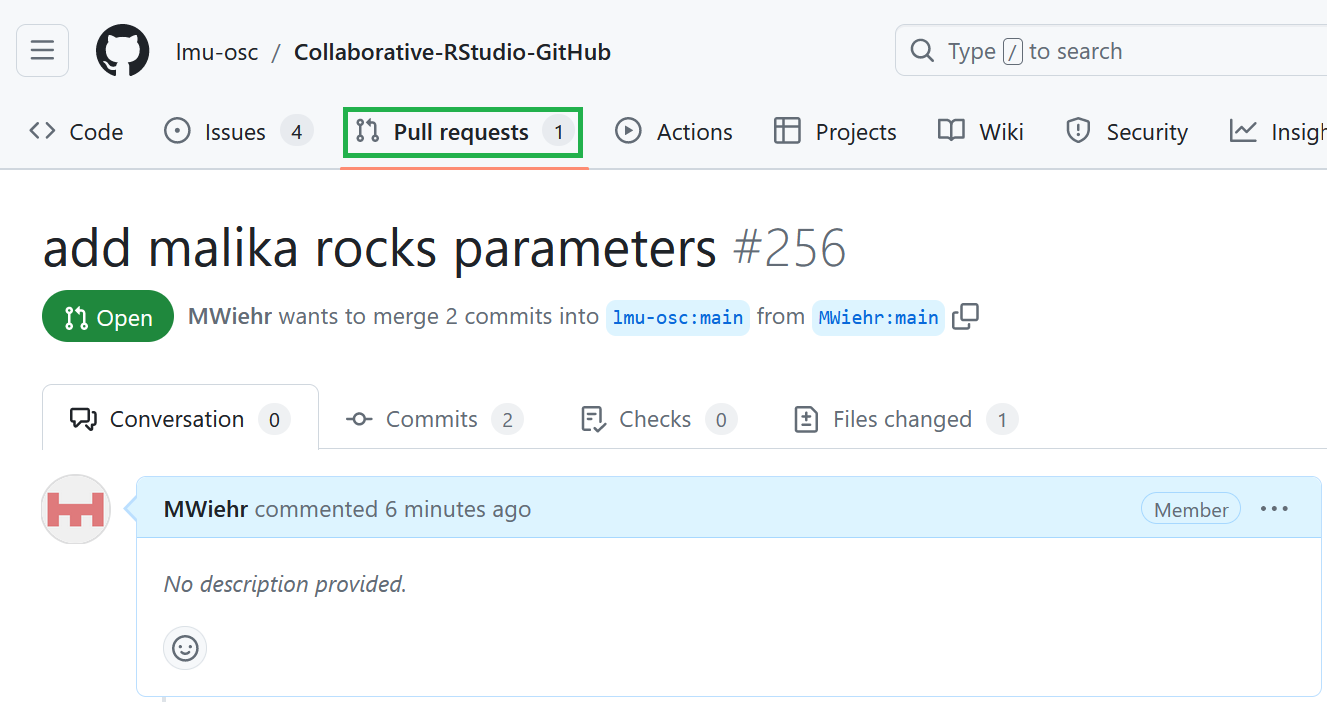
\includegraphics[keepaspectratio]{OS-M3-S5-GitHub-slides_files/mediabag/created-pull-request.png}}
\end{center}

\begin{itemize}
\tightlist
\item
  You should see a conversation tab around your pull request in the
  original repository.
\end{itemize}

\textbf{Presenter Notes}: Add a message describing the changes you made.
Again, you can just state what you added. Now click ``Create pull
request''. In the original repository, you should now see a conversation
tab around the ``Pull request'' button.

\begin{center}\rule{0.5\linewidth}{0.5pt}\end{center}

\subsection{Merge changes}\label{merge-changes}

To \textbf{merge changes} means to combine updates from different
branches or contributors into one unified version of the project.

\begin{itemize}
\tightlist
\item
  Brings everyone's contributions together.
\item
  Ensures new work integrates smoothly with the main branch.
\item
  Helps resolve overlapping edits or conflicts between files.
\end{itemize}

\textbf{Presenter Notes}: Now that the changes have been made and you
opened a pull request, the next step is for those changes to be reviewed
and incorporated into the main branch. This is what is meant by
``merge'' because the contributions from the different collaborators are
merged into the one project that everyone is working on. How does this
contribute towards collaboration? This brings the contributions together
in one place, ensures new work integrates smoothly with the main branch,
and will make overlapping edits or conflicts between files visible so
you can go in and resolve them.

\begin{center}\rule{0.5\linewidth}{0.5pt}\end{center}

\subsection{How to merge changes}\label{how-to-merge-changes}

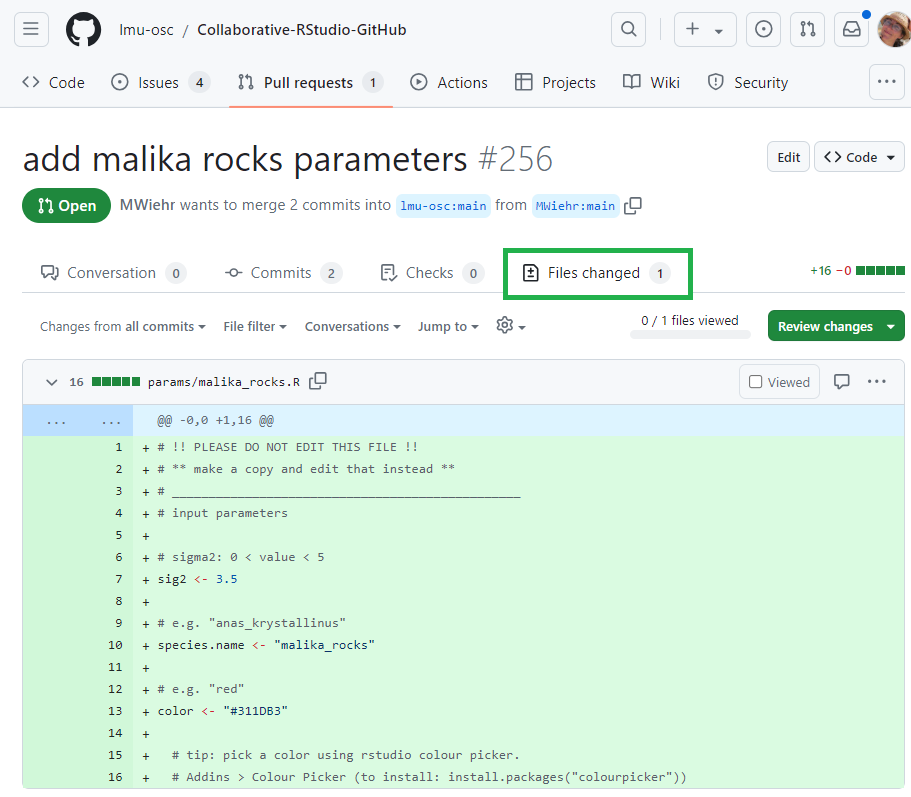
\includegraphics[width=0.8\linewidth,height=\textheight,keepaspectratio]{OS-M3-S5-GitHub-slides_files/mediabag/files-changed.png}

The owner of the main repository:

\begin{itemize}
\tightlist
\item
  Goes to their ``\texttt{Pull\ requests}'' tab to inspect the changed
  files
\item
  Ensures that the parameters were inputted correctly so as to not break
  down their code down the line
\end{itemize}

\begin{tcolorbox}[enhanced jigsaw, colbacktitle=quarto-callout-note-color!10!white, opacityback=0, leftrule=.75mm, colback=white, opacitybacktitle=0.6, colframe=quarto-callout-note-color-frame, title=\textcolor{quarto-callout-note-color}{\faInfo}\hspace{0.5em}{What's happening here?}, left=2mm, titlerule=0mm, toptitle=1mm, breakable, bottomtitle=1mm, arc=.35mm, rightrule=.15mm, bottomrule=.15mm, toprule=.15mm, coltitle=black]

In this example, the file ``malika\_rocks.R'' is being reviewed to then
be added to the ``\texttt{params}'' sub-folder in the main repository
project files.

\end{tcolorbox}

\textbf{Presenter Notes}: If you are the owner of the repository and
will merge files, you must first click on the ``Pull requests'' tab and
inspect the files there. Take one and check that everything was done
correctly so it's ready to merge.

\textbf{Instructor Notes}: First go through the slides of this section
to see how to merge changes, then do a live demonstration using the
changes they made to the Example Project. For this session, the
instructor created the GitHub repository and therefore is the one to
review and merge the changes. But it is still important for the learners
to learn HOW to merge changes for when they begin projects of their own.

\begin{center}\rule{0.5\linewidth}{0.5pt}\end{center}

\subsection{How to merge changes}\label{how-to-merge-changes-1}

\pandocbounded{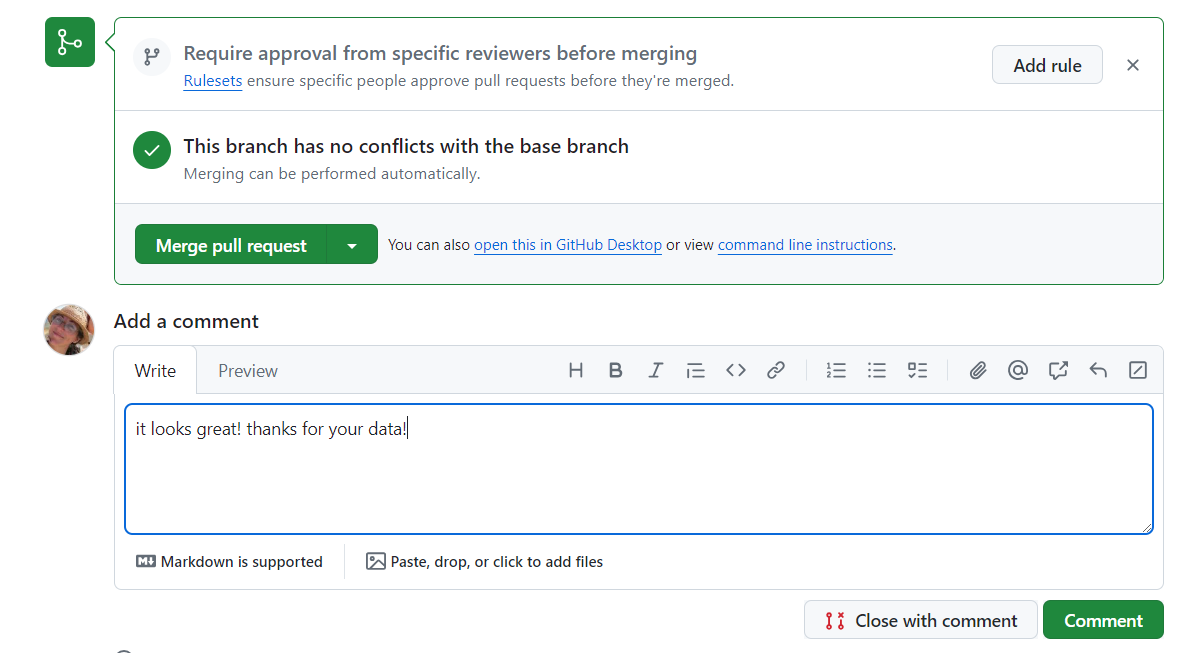
\includegraphics[keepaspectratio]{OS-M3-S5-GitHub-slides_files/mediabag/comment-and-merge.png}}

If everything looks fine, the owner will:

\begin{itemize}
\tightlist
\item
  Go back to the ``\texttt{Pull\ request}'' tab
\item
  Write a comment
\item
  Merge the \textbf{pull request} and \textbf{confirm the merge}
\end{itemize}

\textbf{Presenter Notes}: If everything looks fine, go back to the
``Pull request'' tab, leave a comment (this is optional), and click on
``Merge pull request'' then ``Confirm the merge''. And now that file
that was inspected is now incorporated into the project files in main
repository.

\begin{center}\rule{0.5\linewidth}{0.5pt}\end{center}

\subsection{How to merge changes}\label{how-to-merge-changes-2}

\textbf{Now let's see all the contributions work together!}

\pandocbounded{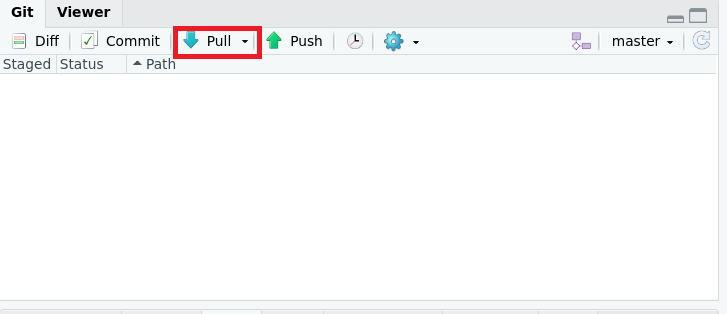
\includegraphics[keepaspectratio]{OS-M3-S5-GitHub-slides_files/mediabag/pull.png}}

\begin{itemize}
\tightlist
\item
  The \textbf{owner of the main repository} will pull the new
  contributed files from GitHub into their local repository using the
  ``\texttt{Pull}'' button in \textbf{RStudio}.
\end{itemize}

\begin{tcolorbox}[enhanced jigsaw, colbacktitle=quarto-callout-note-color!10!white, opacityback=0, leftrule=.75mm, colback=white, opacitybacktitle=0.6, colframe=quarto-callout-note-color-frame, title=\textcolor{quarto-callout-note-color}{\faInfo}\hspace{0.5em}{What should I see?}, left=2mm, titlerule=0mm, toptitle=1mm, breakable, bottomtitle=1mm, arc=.35mm, rightrule=.15mm, bottomrule=.15mm, toprule=.15mm, coltitle=black]

All the contributions that were merged into this repository should show
up in the `Params' sub-folder in the local repository.

\end{tcolorbox}

\textbf{Presenter Notes}: Let us see how all the contributions are
integrated into a single document. First, the owner of the main
repository needs to pull all the files that were pushed by the other
contributors so that all the new files will be on the local copy of the
repository.

\textbf{Instructor Notes}: The instructor (that is, the owner of the
main repository) will perform this task to pull the changes made by the
learners into the main repo.

\begin{center}\rule{0.5\linewidth}{0.5pt}\end{center}

\subsection{How to merge changes}\label{how-to-merge-changes-3}

\begin{center}
\pandocbounded{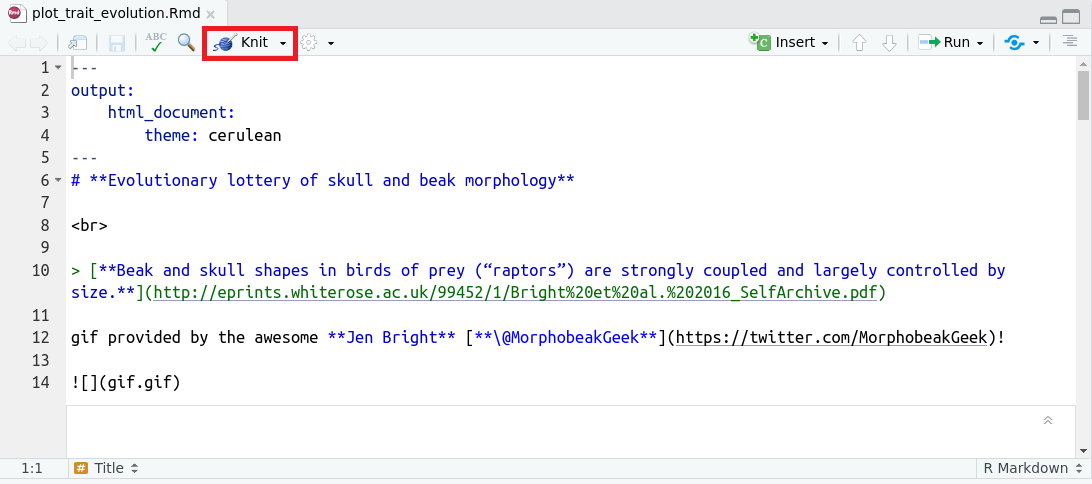
\includegraphics[keepaspectratio]{OS-M3-S5-GitHub-slides_files/mediabag/knit.png}}
\end{center}

\begin{itemize}
\tightlist
\item
  Then, the owner will locate and open the
  ``\texttt{plot-trait-evolution.Rmd}'' file in the repository which
  sources all the contributed files.
\item
  Once opened, they will click the ``\texttt{Knit}'' button on the
  toolbar to generate plots and figures based on the parameters that
  were contributed.
\end{itemize}

\begin{tcolorbox}[enhanced jigsaw, colbacktitle=quarto-callout-note-color!10!white, opacityback=0, leftrule=.75mm, colback=white, opacitybacktitle=0.6, colframe=quarto-callout-note-color-frame, title=\textcolor{quarto-callout-note-color}{\faInfo}\hspace{0.5em}{What does \texttt{Knit} do?}, left=2mm, titlerule=0mm, toptitle=1mm, breakable, bottomtitle=1mm, arc=.35mm, rightrule=.15mm, bottomrule=.15mm, toprule=.15mm, coltitle=black]

\textbf{Knitting} a Rmarkdown file means rendering the Rmarkdown code.
This integrates the R code and Markdown code into a defined format (for
example: an html file).

\end{tcolorbox}

\textbf{Presenter Notes}: After pulling everyone's changes, the owner
opens the main R Markdown file called ``plot-trait-evolution.Rmd.'' This
file combines all the contributed scripts. By clicking the `Knit'
button, RStudio runs the code and produces plots and figures that
include everyone's new parameters.

\begin{center}\rule{0.5\linewidth}{0.5pt}\end{center}

\subsection{How to merge changes}\label{how-to-merge-changes-4}

\pandocbounded{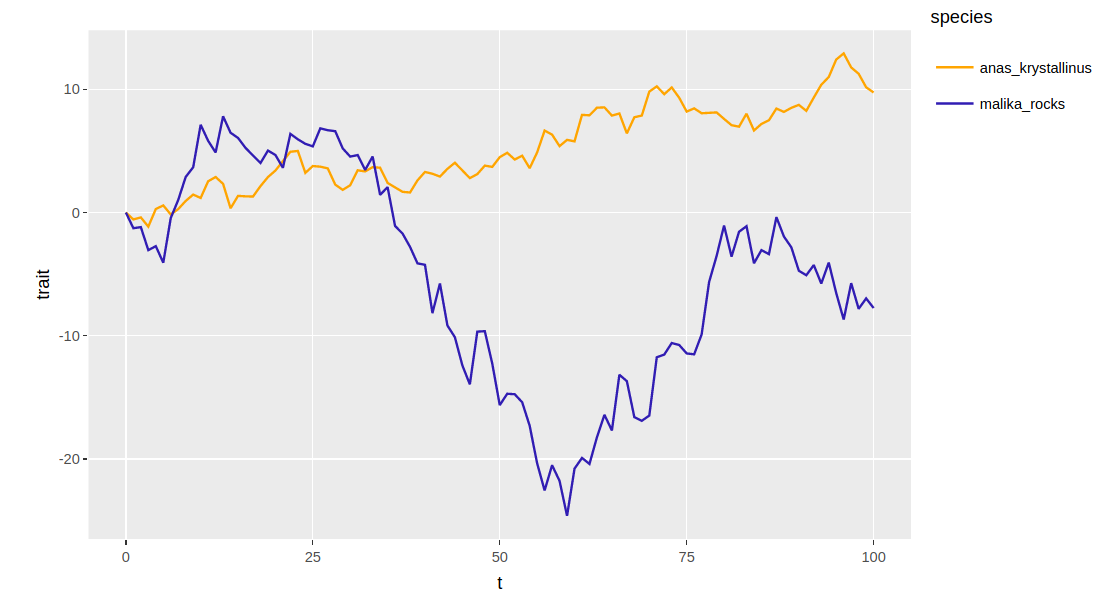
\includegraphics[keepaspectratio]{OS-M3-S5-GitHub-slides_files/mediabag/plot.png}}

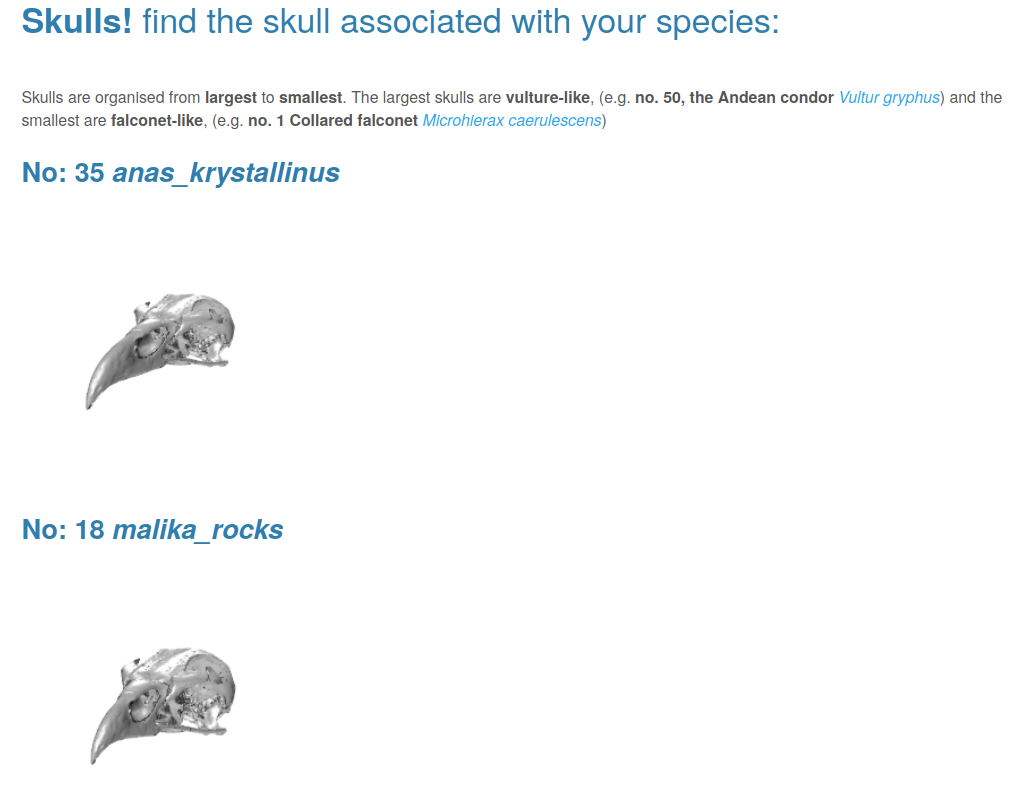
\includegraphics[width=0.7\linewidth,height=\textheight,keepaspectratio]{OS-M3-S5-GitHub-slides_files/mediabag/skulls.png}

\begin{itemize}
\tightlist
\item
  An \textbf{html document} will appear that shows the contributions
  plotted altogether on a line graph and images of skulls under the
  names of the species.
\end{itemize}

\textbf{You did it! You collaborated on GitHub!}

\textbf{Presenter Notes}: When the owner knits the R Markdown file, an
HTML report appears showing everyone's contributions together with each
species' trait evolution plotted on the same line graph, along with
their matching skull images. We can now see that all the collaborators'
work successfully came together through GitHub!

\begin{center}\rule{0.5\linewidth}{0.5pt}\end{center}

\subsection{Merge changes - live demo!}\label{merge-changes---live-demo}

Now let's see what that looks like for this project with a \textbf{live
demonstration} using your contributions!

\textbf{Presenter Notes}: Now that we know what to do, let's see it in
action with a live demonstration! We will merge changes in one or more
forks with the main repository project files via the pull requests.

\textbf{Instructor Notes}: Do a live demonstration of merging some
changes. Depending on the size of the class, it may be too
time-consuming to review and merge the changes from each individual
learner. - For this particular project, the things you want to check for
during your review is that each new file has the 3 elements in the
correct format: `sig2' is a numerical value between 1-5 with no
quotation marks; `species.name' has quotation marks; `color' is a hex
code starting with a \# followed by 6 characters and is in quotation
marks. Errors here can break the code. - When you open the
``plot-trait-evolution.Rmd'' file, you would have to install and load
the necessary packages before hitting `Knit'- the packages are detailed
in the file itself. - Note this demo is only suitable for a class-room
setting.

\begin{center}\rule{0.5\linewidth}{0.5pt}\end{center}

\subsection{Pull upstream}\label{pull-upstream}

To \textbf{pull upstream} means to update your local or forked
repository with the latest changes from the original (upstream)
repository.

\begin{itemize}
\tightlist
\item
  Keeps your local copy aligned with the main project's progress.
\item
  Prevents outdated or conflicting edits when working in teams.
\item
  Encourages synchronization across all contributors.
\end{itemize}

\textbf{Presenter Notes}: Even after you pushed your changes and it was
merged into the main branch, the project may still be ongoing or your
local and remote copied repositories may not have the contributions from
the other collaborators. This is why you should pull upstream to update
your local or forked repository with the latest changes from the
original repo. How does this contribute towards collaboration? It keeps
your local copy updated with the changes in the main project, prevents
outdated or conflicting edits, and synchronizes work across each
contributor.

\textbf{Instructor Notes}: Back to the learners! Here the learners will
perform this task as they must now pull the changes that the instructor
merged into the main repository. This means they will incorporate the
changes into their individual copies of the project, emphasize that this
is a process to keep all their copies up to date with the changes and
contributions made.

\begin{center}\rule{0.5\linewidth}{0.5pt}\end{center}

\subsection{Practical exercise 6: Pull}\label{practical-exercise-6-pull}

\begin{itemize}
\tightlist
\item[$\square$]
  In \textbf{RStudio}, go to the ``\texttt{Terminal}'' tab
\item[$\square$]
  Enter the following command:
\end{itemize}

\begin{Shaded}
\begin{Highlighting}[]
\NormalTok{git checkout main}
\end{Highlighting}
\end{Shaded}

\begin{tcolorbox}[enhanced jigsaw, colbacktitle=quarto-callout-note-color!10!white, opacityback=0, leftrule=.75mm, colback=white, opacitybacktitle=0.6, colframe=quarto-callout-note-color-frame, title=\textcolor{quarto-callout-note-color}{\faInfo}\hspace{0.5em}{\texttt{git\ checkout}}, left=2mm, titlerule=0mm, toptitle=1mm, breakable, bottomtitle=1mm, arc=.35mm, rightrule=.15mm, bottomrule=.15mm, toprule=.15mm, coltitle=black]

This command sets the branch to the one you want to pull the
modifications from. In this case, you want to pull the changes from the
\emph{main branch} of the \emph{remote main repository} into your the
\emph{main branch} of your \textbf{local repository}.

\end{tcolorbox}

\textbf{Presenter Notes}: If you want the changes or updates to appear
on your fork on GitHub, you need to first pull the updates from the main
repository directly into your local repository, not to your remote fork
just yet. When the changes are pulled into your local copy, then you can
push the changes to your remote fork. To do this, we go back into
RStudio and go to the ``Terminal'' tab and enter the given git command.
The ``git checkout main'' command sets the main branch of the main
repository as the place we want to pull the updates from.

\begin{center}\rule{0.5\linewidth}{0.5pt}\end{center}

\subsection{Practical exercise 6:
Pull}\label{practical-exercise-6-pull-1}

\begin{itemize}
\tightlist
\item[$\square$]
  In the \textbf{RStudio} ``\texttt{Terminal}'', enter the command to
  pull the original repo and branch following this format:
\end{itemize}

\begin{Shaded}
\begin{Highlighting}[]
\NormalTok{git pull git@github.com:ORIGINAL\_OWNER/ORIGINAL\_REPOSITORY.git}
\end{Highlighting}
\end{Shaded}

\begin{tcolorbox}[enhanced jigsaw, colbacktitle=quarto-callout-warning-color!10!white, opacityback=0, leftrule=.75mm, colback=white, opacitybacktitle=0.6, colframe=quarto-callout-warning-color-frame, title=\textcolor{quarto-callout-warning-color}{\faExclamationTriangle}\hspace{0.5em}{How to properly format this command?}, left=2mm, titlerule=0mm, toptitle=1mm, breakable, bottomtitle=1mm, arc=.35mm, rightrule=.15mm, bottomrule=.15mm, toprule=.15mm, coltitle=black]

Replace the ``\texttt{ORIGINAL\_OWNER}'' with the name of the GitHub
account that owns the main repository. Replace
``\texttt{ORIGINAL\_REPOSITORY}'' with the name of the main repository
that has the original project files.

\end{tcolorbox}

\textbf{Presenter Notes}: Next, we type this command to pull the
original repository and branch we wish to obtain locally. Follow the
format but replace ``ORIGINAL\_OWNER'' and ``ORIGINAL\_REPOSITORY''.
Here's an example of what it looks like when these two commands are
executed successfully.

\begin{center}\rule{0.5\linewidth}{0.5pt}\end{center}

\subsection{Practical exercise 6:
Pull}\label{practical-exercise-6-pull-2}

This is an example.

\textbf{Presenter Notes}: Let's look at this example: first there is the
``git checkout main'' command to set the main branch of the main
repository as the place to pull the changes from. Then the ``git pull
git@github.com:'' command is followed by the owner and repository name.
In this case the original owner is ``lmu-osc'' and the orginal
repository is ``Collaborative-RStudio-GitHub.git''.

\begin{center}\rule{0.5\linewidth}{0.5pt}\end{center}

\subsection{Practical exercise 6:
Pull}\label{practical-exercise-6-pull-3}

\begin{itemize}
\tightlist
\item[$\square$]
  In \textbf{RStudio}, check the ``\texttt{Files}'' tab and open the
  ``\texttt{params}'' sub-folder
\item[$\square$]
  In the ``\texttt{params}'' sub-folder, check that the new R files with
  the parameter contributions are appearing (the ones that were merged)
\item[$\square$]
  To push these new parameter contributions into your remote fork on
  \textbf{GitHub}, you can also do so by entering the following command
  into the terminal
\end{itemize}

\begin{Shaded}
\begin{Highlighting}[]
\NormalTok{git push}
\end{Highlighting}
\end{Shaded}

\begin{figure}[H]

{\centering \pandocbounded{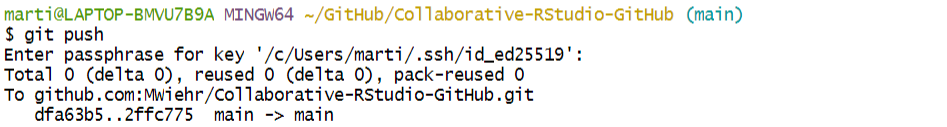
\includegraphics[keepaspectratio]{OS-M3-S5-GitHub-slides_files/mediabag/final-push.png}}

}

\caption{This is an example.}

\end{figure}%

\textbf{Presenter Notes}: Earlier we merged some new R files containing
unique parameters into the main repository. After pulling upstream,
these files should now be showing up in your ``File'' tab in RStudio,
this means that they are now on your local copy. To also have them
appear on your fork on GitHub you can push them using a simple Git
command: git push. Enter this into the terminal to execute it. Then
check your fork on GitHub to make sure the new files are also appearing
in the ``params'' sub-folder there.

\begin{center}\rule{0.5\linewidth}{0.5pt}\end{center}

\subsection{And that is it!}\label{and-that-is-it}

\textbf{You just completed the entire workflow!}

\begin{itemize}
\tightlist
\item
  You \textbf{started with making a fork} of the main repository with
  the project files to make your changes without affecting anyone else's
  work.
\item
  Then you \textbf{pushed} and had these \textbf{changes merged} into
  the main repository.
\item
  Lastly, you \textbf{pulled these changes} so that your copies (remote
  and local) can stay updated with the changes made.
\end{itemize}

\textbf{Presenter Notes}: Great job, you have completed a full GitHub
collaboration cycle. You forked the main repository, made and committed
your own changes, pushed them for review, and finally pulled the merged
updates back into your local copy. This is the same workflow used in
real research collaborations.

\begin{center}\rule{0.5\linewidth}{0.5pt}\end{center}

\subsection{Recap}\label{recap}

\textbf{What actions did we learn in today's lesson?}

\begin{itemize}
\tightlist
\item
  \textbf{Fork a repo}: make your own copy on GitHub
\item
  \textbf{Clone the repo}: bring it to your local computer
\item
  \textbf{Commit}: make changes locally
\item
  \textbf{Push}: upload those changes to your fork on GitHub
\item
  \textbf{Pull request}: propose those changes to the main/original repo
\item
  \textbf{Merge}: the project owner merges your pull request into the
  main branch
\item
  \textbf{Pull upstream}: after the merge, you pull the updated main
  branch from the original repo to sync your local copy
\end{itemize}

\textbf{Presenter Notes}: Here is a quick recap of the full GitHub
workflow we practiced today. You learned how to fork a repository, clone
it to your local device, make and commit changes, push them to your fork
on GitHub, open a pull request, and finally merge and pull updates.
These are the core steps you can use for collaborative coding in
research.

\begin{center}\rule{0.5\linewidth}{0.5pt}\end{center}

\subsection{Recap activity}\label{recap-activity}

Remember this illustration?

\begin{center}
\pandocbounded{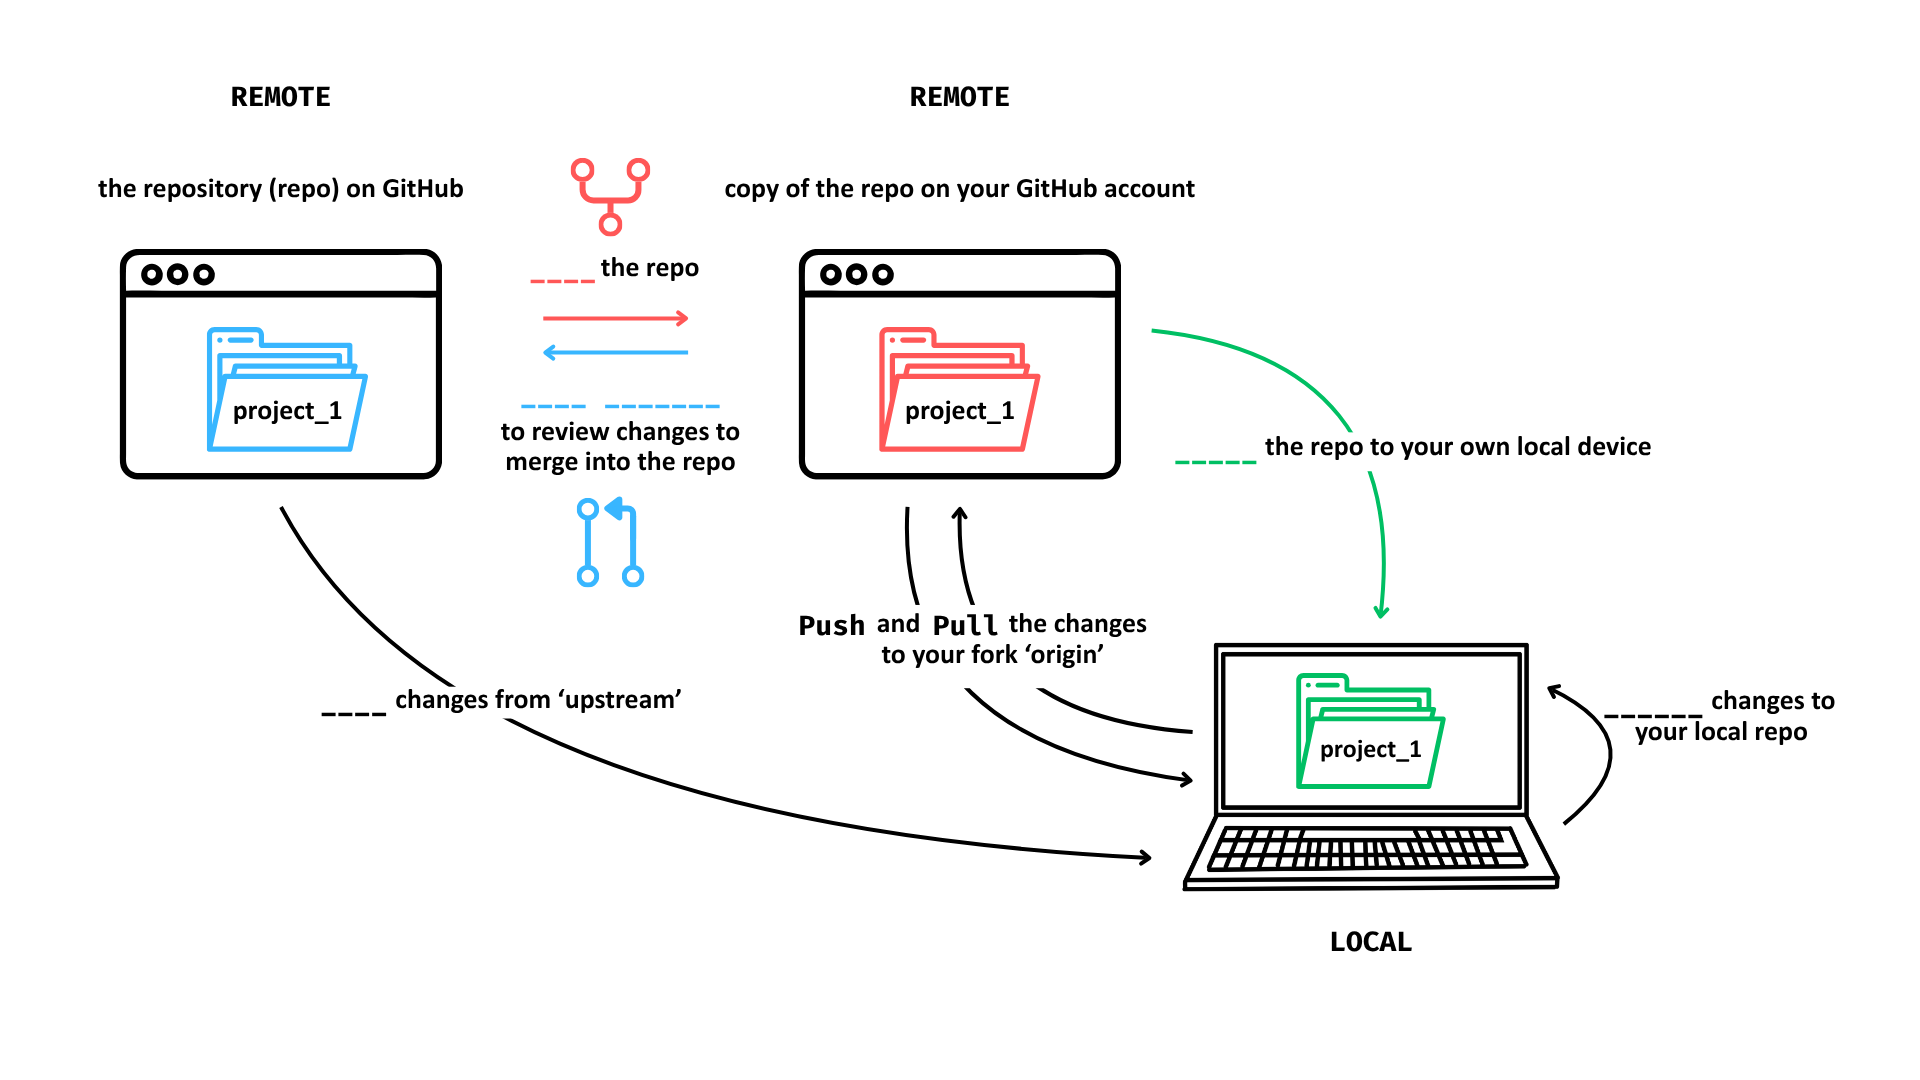
\includegraphics[keepaspectratio]{images/04_Recap_Activity.png}}
\end{center}

\emph{Fill in the missing words with the actions we learned today!}

\textbf{Presenter Notes}: Let's revist this diagram we saw at the
beginning of the lesson. See if you can fill in the missing words with
the actions we used to collaborate on the project today using GitHub.

\begin{center}\rule{0.5\linewidth}{0.5pt}\end{center}

\subsection{Recap activity}\label{recap-activity-1}

\textbf{Check your answers!}

Download the completed diagram

\textbf{Presenter Notes}: Now you can download the original image and
check your answers.

\begin{center}\rule{0.5\linewidth}{0.5pt}\end{center}

\subsection{Collaborative coding with
GitHub}\label{collaborative-coding-with-github}

Now that you have all gained some experience working collaboratively
using GitHub, let us reflect with some questions:

\textbf{1. How can collaborative coding with GitHub be useful?}

\textbf{2. What potential problems could still arise using this
workflow?}

\textbf{Presenter Notes}: So, you have seen the full workflow in action
and practiced collaborative coding facilitated by GitHub. Let's reflect
further on this experience, how could this be useful? Think about how
this kind of collaborative coding can support your own research and
projects.

\textbf{Instructor Notes}: The aim of this slide is to work out the
relevance of the topic to your learners. In an interactive setting,
discuss how the new skills could be applied in practise with specific
examples. Examine downfalls and practical obstacles. Invite the learners
to relate the practice from today's session to their own experiences.
This gives them a chance to think about how they may apply their
new-found skills in collaborative coding with GitHub to their existing
or upcoming projects. Then, ask learners to share or discuss in groups
what they've come up with. Possible answers: - Version control means
every change is tracked, so mistakes can be undone easily. - It allows
multiple people to work on the same project at once, even from different
locations, without overwriting each other's work. - By sharing code
through repositories, others can reproduce your analyses and see exactly
how results were produced. This strengthens both collaboration and
scientific transparency.

Some potential issues:

\begin{itemize}
\item
  Merge conflicts: When two people edit the same part of a file, Git
  cannot automatically merge the changes, leading to so-called merge
  conflicts.
\item
  Unclear commit messages: Inconsistent or unclear commit messages or
  too many small commits can make it hard to track changes.
\item
  Pull request overload: Too many open pull requests can slow down
  reviews and lead to bottlenecks.
\item
  Communication issues: Lack of communication about who is working on
  what can lead to duplicated effort or conflicts.
\end{itemize}

\begin{center}\rule{0.5\linewidth}{0.5pt}\end{center}

\subsection{Take-home message}\label{take-home-message}

Consider the following question:

\textbf{If you had to explain to a new teammate why using GitHub for
collaboration is valuable, what key ideas from today would you talk
about?}

\textbf{Presenter Notes:} Let's think about a take-home message from
today's lesson. Take a few moments and consider the question on the
slide and then let's discuss it.

\begin{center}\rule{0.5\linewidth}{0.5pt}\end{center}

\subsection{Git from the terminal}\label{git-from-the-terminal}

\begin{itemize}
\tightlist
\item
  Several actions in collaborative coding on GitHub can also be
  performed directly using \textbf{Git commands in a so-called terminal}
  instead of using the functions in RStudio.
\end{itemize}

\begin{tcolorbox}[enhanced jigsaw, colbacktitle=quarto-callout-tip-color!10!white, opacityback=0, leftrule=.75mm, colback=white, opacitybacktitle=0.6, colframe=quarto-callout-tip-color-frame, title=\textcolor{quarto-callout-tip-color}{\faLightbulb}\hspace{0.5em}{What is a \textbf{terminal}?}, left=2mm, titlerule=0mm, toptitle=1mm, breakable, bottomtitle=1mm, arc=.35mm, rightrule=.15mm, bottomrule=.15mm, toprule=.15mm, coltitle=black]

It is a text-based tool where you can type commands to run programs such
as Git. If you downloaded Git for \textbf{Windows}, you can right-click
in a folder \emph{\textgreater{} Show more Options \textgreater{} Git
Bash here} to open Git Bash. On \textbf{MacOS}, you can use the built-in
Terminal by going to \emph{Finder \textgreater{} Applications
\textgreater{} Utilities \textgreater{} Terminal}.

\end{tcolorbox}

\begin{center}\rule{0.5\linewidth}{0.5pt}\end{center}

\subsection{Assignment}\label{assignment}

Here is an activity sheet to learn and practice Git commands \textbf{in
the terminal}:

Download the GitHub activity sheet

\textbf{Instructor Notes}: Design a take home assignment that learners
can complete to strengthen or build on the skills learned in this
session. Make sure to explain the homework assignment and the rationale
behind the homework. - Examine whether/how it will be assessed - Mention
scoring rubrics, if applicable - Design a peer-review system for
assignments to place learners in the role of reviewer and author

A suggestion is to design an assignment giving learners the opportunity
to learn how and practice using Git commands in Git Bash to communicate
with GitHub for actions like cloning, committing, pushing, and pulling.

\begin{center}\rule{0.5\linewidth}{0.5pt}\end{center}

\subsection{To conclude: Survey time!}\label{to-conclude-survey-time}

\begin{center}
\pandocbounded{
\includegraphics[keepaspectratio]{images/00_Particify_Survey_Rooms.png}}
\end{center}

\begin{tcolorbox}[enhanced jigsaw, colbacktitle=quarto-callout-note-color!10!white, opacityback=0, leftrule=.75mm, colback=white, opacitybacktitle=0.6, colframe=quarto-callout-note-color-frame, title=\textcolor{quarto-callout-note-color}{\faInfo}\hspace{0.5em}{Final survey}, left=2mm, titlerule=0mm, toptitle=1mm, breakable, bottomtitle=1mm, arc=.35mm, rightrule=.15mm, bottomrule=.15mm, toprule=.15mm, coltitle=black]

Please complete survey labeled ``OS-M3-S5-GitHub-finishing\_survey''.

\end{tcolorbox}

\textbf{Presenter Notes}: To end this lesson, let's use this survey to
see where we stand in our understanding of using GitHub and what we can
focus on more moving forward to become more proficient in using it for
collaborative work. Scan the QR code once more and go to the
OS-M3-S5-GitHub-finishing\_survey.

\emph{Instructor Notes} - Aim: This post-submodule survey serves to
examine learners' current knowledge about the sumodule's topic. - Use
free survey software such as or other survey software (particify, formR)
to establish the following questions (these are examples that can be
adapted to suit your needs):

\begin{center}\rule{0.5\linewidth}{0.5pt}\end{center}

\textbf{Which of the following concepts or skills do you feel MOST
confident about in relation to Git and GitHub? (Select all that apply)}

\begin{enumerate}
\def\labelenumi{\alph{enumi}.}
\item
  Forking a repository and working on my own copy.
\item
  Cloning a repository from GitHub to my local machine.
\item
  Making commits and writing meaningful commit messages.
\item
  Pushing local changes to a remote repository.
\item
  Pulling or fetching updates from a remote repository.
\item
  I am still not sure about any of these concepts.
\end{enumerate}

\begin{center}\rule{0.5\linewidth}{0.5pt}\end{center}

\textbf{On a scale of 1 to 5, how comfortable are you right now with
using Git and GitHub for collaborative coding and version control? (1 =
Not comfortable at all, 5 = Very comfortable)}

\begin{enumerate}
\def\labelenumi{\alph{enumi}.}
\item
  1
\item
  2
\item
  3
\item
  4
\item
  5
\end{enumerate}

\begin{center}\rule{0.5\linewidth}{0.5pt}\end{center}

\textbf{When you worked collaboratively on this GitHub project, what
aspect did you find most challenging?}

\begin{enumerate}
\def\labelenumi{\alph{enumi}.}
\item
  Understanding Git commands (commit, push, pull)
\item
  Remembering all the steps
\item
  Navigating the GitHub interface
\item
  Other
\end{enumerate}

\begin{center}\rule{0.5\linewidth}{0.5pt}\end{center}

\subsection{Discussion of survey
results}\label{discussion-of-survey-results-1}

What do we see in the results and how do they compare to the previous
ratings?

\textbf{Presenter Notes}: Now that you've completed both the pre- and
post-module survey, let's compare the results to see where we began and
how we've made progress. This is also a good time to raise any concerns
or clarify any concepts you may not have understood fully.

\textbf{Instructor Notes}: Aim: Briefly examine the answers given to
each question interactively with the group. Compare and highlight
specific differences in answers between pre- and post-survey answers

\begin{center}\rule{0.5\linewidth}{0.5pt}\end{center}

\subsection{References}\label{references}

\begin{itemize}
\tightlist
\item
  Krystalli, A. (2024). Collaborative coding with GitHub and RStudio.
  \href{https://lmu-osc.github.io/Collaborative-RStudio-GitHub/}{lmu-osc.github.io/Collaborative-RStudio-GitHub}
\end{itemize}

\begin{center}\rule{0.5\linewidth}{0.5pt}\end{center}

\section{\texorpdfstring{Thanks! }{Thanks!  }}\label{thanks}

See you next class :)

\begin{center}\rule{0.5\linewidth}{0.5pt}\end{center}

\subsection{Pedagogical add-on tools for
instructors}\label{pedagogical-add-on-tools-for-instructors}

\begin{itemize}
\tightlist
\item
  The contents are adapted from the
  \href{https://lmu-osc.github.io/Collaborative-RStudio-GitHub/}{LMU
  OSC's Collaborative coding with GitHub and RStudio tutorial}.
\item
  One-Minute Paper is a quick reflective activity where learners spend
  about a minute writing brief responses to summarize what they learned.
  Check out the
  \href{https://www.rochester.edu/college/teaching/teaching-guidance/one-minute-paper.html}{University
  of Rochester's Teaching Center Page} to learn more about it.
\item
  Pair theoretical aspects with practical exercises and group
  discussions according to the Think-Pair-Share style and according to
  Cognitive Load Theory (Sweller, 1980).
\end{itemize}

\begin{center}\rule{0.5\linewidth}{0.5pt}\end{center}

\subsection{Additional related
content}\label{additional-related-content}

Here are some topics that are related to this session

\begin{itemize}
\tightlist
\item
  If you already have a project using RStudio that you now want to begin
  collaborative coding with, you can follow
  \href{https://www.youtube.com/watch?v=bUoN85QvC10}{this video on how
  to connect existing RStudio projects with GitHub}.
\item
  \href{https://github.com/features/copilot}{GitHub Copilot} is GitHub's
  AI tool (developed with OpenAI) to assist developers by suggesting
  code, completing functions, and explaining snippets directly inside
  editors.
\end{itemize}

\begin{center}\rule{0.5\linewidth}{0.5pt}\end{center}

\subsection{Attribution and license details
UNFINISHED}\label{attribution-and-license-details-unfinished}

\begin{itemize}
\item
  This slide should contain information about the license and
  attribution details of this current set of slides.
\item
  The default for the created materials is
  \href{https://creativecommons.org/licenses/by/4.0/}{CC-BY-SA 4.0}

  \begin{itemize}
  \tightlist
  \item
    = Creative Commons license that allows others to \textbf{share,
    adapt, and build upon} the original work
  \item
    \textbf{only} if they attribute the creator and also share their new
    work under the \textbf{same terms}
  \item
    allows for both \textbf{commercial and non-commercial} use of the
    licensed material
  \end{itemize}
\item
  Components of attributions:

  \begin{itemize}
  \tightlist
  \item
    \texttt{Title}
  \item
    \texttt{Author}
  \item
    \texttt{Source}
  \item
    \texttt{License}
  \end{itemize}
\end{itemize}

\begin{center}\rule{0.5\linewidth}{0.5pt}\end{center}




\end{document}
